\chapter{Development}

\label{ch:conclusions}

\section{Introduction}

As explained in the design chapter, this project includes three deliverables. So the development will include; a Mac app dashboard, Perfect web-server and CocoaPods framework. Using the ”tree-shaped” methodology, the web-server was split up into their separate sections which include development, testing, and run. Then each service was design, developed and testing before moving up the tree. The development was broken up into phases, this way the project is kept on track on what has been completed and left to do.

\begin{enumerate}
  \item Services Development
  \item Integrate into Live App
  \item Web server 
  \item Dashboard Development
  \item CocoaPod Framework 
\end{enumerate}

As this project methodology is based on Test Driven Development (TDD) approach, the services were developed first and tested before adding to the project. Once these services have cleared testing individually, they were integrated into the DIT-Timetable app explained later, this was to ensure how the new services were developed would pass Apples pre-publishing tests. Once this was accomplished, the dashboard was designed next to view the services in an interface. Then lastly the services were developed into an SDK to be used in any mobile application.

\section{Project Management}

Good software project management is essential in developing and delivery of software projects. Software development is often difficult to estimate the time required to complete the project, especially when using new technologies. Project milestones can be used to monitor the development progress of the project at certain key points. Above includes the list of the key points within the project. 

Each point had its time frame; this kind of project can lead to expanding to including more services and tools, so sticking to the list will help be on schedule.This project differs from a commercial project, in that the project manager, designer, developer and tester are all the same person. And with any project, testing plays a significant role in software development and can easily be left out.

\section{Services Development}

Each service had it's own or where possible shared Perfect server application along with Playground app. This made is easy to decide whether or not it was possible to implement each service into the project. For some of the services, the same Perfect web-server was used and able to be adapted to accommodate the requests needed. 

\paragraph{Setup} 

Before any development was started, some services were required to be setup. Perfect web-server developers provide an ”assistant app” to help with the configuration and include any required packages needed to develop the API. The list of packages for the project includes the following:

\begin{enumerate}
  \item https://github.com/PerfectlySoft/Perfect-Turnstile-MongoDB.git
  
  -Used to provide functionality to interact with MongoDB database, and provide authentication when requests come to the server.
  \item https://github.com/PerfectlySoft/Perfect-RequestLogger.git
  
  -Provides the web-server with a logging system.
  \item https://github.com/hkellaway/Gloss.git
  \item https://github.com/PerfectlySoft/Perfect-Notifications.git
  
  -Aid with the push notifications.
  \item https://github.com/PerfectlySoft/Perfect-SMTP.git
  
  -To add capability of sending e-mails
  \item https://github.com/PerfectlySoft/Perfect-Zip.git
  
  -To zip backups folders, when sending to a remote location.
\end{enumerate}

After the Perfect web-server was setup, the mongoDB database was required to installed locally. This was done by running the following commands in list \ref{lst:mongodb}

\lstinputlisting[label={lst:mongodb}, language=Bash, caption=MongoDB setup]{development/code/mongo.m}


\lstinputlisting[label={lst:playground},language=Swift, caption=Playgrounds setup]{development/code/playground.m}

The request over HTTP will be made using asynchronous; this does not block the interface while the request which can be time-consuming. The interface should not be blocked, making the user wait. To be able to run asynchronous requests in the playground apps, the following lines of code in Listing \ref{lst:playground} is required to the top of the file.

\subsubsection{Database storage}

The database storage section was split up into two parts of the development. 

\begin{enumerate}
  \item Object-relational mapping (ORM)
  \item Storage - how to send the objects to store persistently
\end{enumerate}

\paragraph{ORM}

The database storage service required an object-relational mapping (ORM) which is a powerful method for designing and querying database models at the conceptual level, where the application is described in terms easily understood by non-technical database developers. It is a technique for converting data between incompatible type systems in object-oriented programming languages. The ORM was developed using Playground tool, where the creation of objects and parsing into JSON objects was done. The functionality of the ORM is to create a new object, parse it and send to the server, and be able to bring all objects back from the server.

This was developed using protocols and protocol extension. Protocols as Apple states "defines a blueprint of methods, properties, and other requirements that suit a particular task or piece of functionality." and extensions are "new functionality to an existing class, .., protocol type.". \cite{protocol} A protocol called \textit{TBJSONSerializable} was developed as seen in Listing \ref{lst:protocol_ext}

\lstinputlisting[label={lst:protocol_ext},language=Swift, caption=Protocol]{development/code/protocol_ext.m}

The first protocol \textit{TBJSONRepresentable} just states that this variable \textit{TBJSONRepresentation} has to be used in any class or protocol conforming to that protocol. Inside the \textit{TBJSONSerializable} protocol, we have two methods that any class or structure used throughout any mobile application are required to used. The \textit{TBJSON} to a type alias that is a dictionary, which holds the JSON objects which will be used when parsing. Next the protocol extension was developed, where the objects will be parsed into a dictionary type form that then can easily be parsed in JSON. In Listing \ref{lst:TBJSONSerializable} illustrates how the objects are parsed.

\lstinputlisting[label={lst:TBJSONSerializable},language=Swift,caption=TBJSONSerializable]{development/code/TBJSONSerializable.m}

In Listing \ref{lst:TBJSONSerializable}, the \textit{TBJSONRepresentation} variable contains a switch case to loop through the mirrored object properties; which is a representation of the sub-structure. Then each property type such as String, Int or Dictionary, and depending on the type can be parsed into an AnyObject type and assigned to the dictionary with the key being the name of the variable.

The design also stated that in retrieving objects, functionality is to be in placed to parse back to objects. A list of functions was implemented to parse each value back to the desired type using protocol extension to type dictionary and method chaining. The method chaining speeds the development time for the developer, without needing to find the correct type first. An example of this is in Listing \ref{lst:tryConvert} which takes the parameter of the key and tries to parse the value in two ways. First, if the value if of type integer, it will return that value, but if it is of type String, it will convert a string to integer and return the new value.

\lstinputlisting[label={lst:tryConvert},language=Swift, caption=Dictionary]{development/code/tryConvert.m}

\paragraph{Storage}

As part of the project architecture with regarding storage, any structure should have the functionality to send the object to the server, and retrieve without the need to create another function to setup and communicate over HTTP. As described in the design chapter, all structures conforming to the protocol will be able to send and retrieve the object/s between the server and the application. JSON is used in the transfer of data, a format in which both server and client can understand. JSON objects are simply just dictionaries where each value is an object of some type. The following table \ref{tb:object} illustrates the library commands to send and retrieve objects between the cloud storage. The \textit{T} in the return column means that this function return type is of a particular type. In the following examples will be returning type \textit{TBJSONSerializable} which is our protocol.

\begin{table}[!h]
\centering
\caption{My caption}
\label{tb:object}
\begin{tabular}{|c|l|c|l|}
\hline
\rowcolor{green!20}
\multicolumn{1}{|l|}{Library Method} & Description & \multicolumn{1}{l|}{Parameters}                                                       & Result            \\ \hline
getFilteredInBackground                                      & \begin{tabular}[c]{@{}l@{}}Retrieves the filtered\\ object\end{tabular} & \begin{tabular}[c]{@{}c@{}}query: {[}String:AnyObject{]}, \\ type:T.Type, \\ appKey: String = ""\end{tabular} & T Object          \\ \hline
getInBackground                                              & Retrieves the object                                                    & \begin{tabular}[c]{@{}c@{}}objectID: String, type:T.Type, \\ appKey: String = ""\end{tabular}                 & T Object          \\ \hline
removeInBackground                                           & Removes the object                                                      & objectID: String, appKey: String = ""                                                                         & Successful/ Error \\ \hline
sendInBackground                                             & \begin{tabular}[c]{@{}l@{}}Update or send the \\ object\end{tabular}    & \multicolumn{1}{l|}{objectID: String, appKey: String = ""}                                                    & Successful/ Error \\ \hline
\end{tabular}
\end{table}

The next table \ref{tb:objects} illustrates returning back array of objects.


\begin{table}[!h]
\centering
\caption{My caption}
\label{tb:objects}
\begin{tabular}{|c|l|c|l|}
\hline
\rowcolor{green!20}
\multicolumn{1}{|l|}{Library Method} & Description & \multicolumn{1}{l|}{Parameters}                                                       & Result            \\ \hline
getFilteredInBackground                                      & \begin{tabular}[c]{@{}l@{}}Retrieves the filtered\\ object\end{tabular} & \begin{tabular}[c]{@{}c@{}}query: {[}String:AnyObject{]}, \\ type:T.Type, \\ appKey: String = ""\end{tabular} & T Objects \\ \hline
getAllInBackground                                           & Retrieves the object                                                    & \begin{tabular}[c]{@{}c@{}}objectID: String, type:T.Type, \\ appKey: String = ""\end{tabular}                 & T Objects \\ \hline
\end{tabular}
\end{table}

\begin{figure}[!h]
    \caption{Storage Sequence Standard}
    \centering
    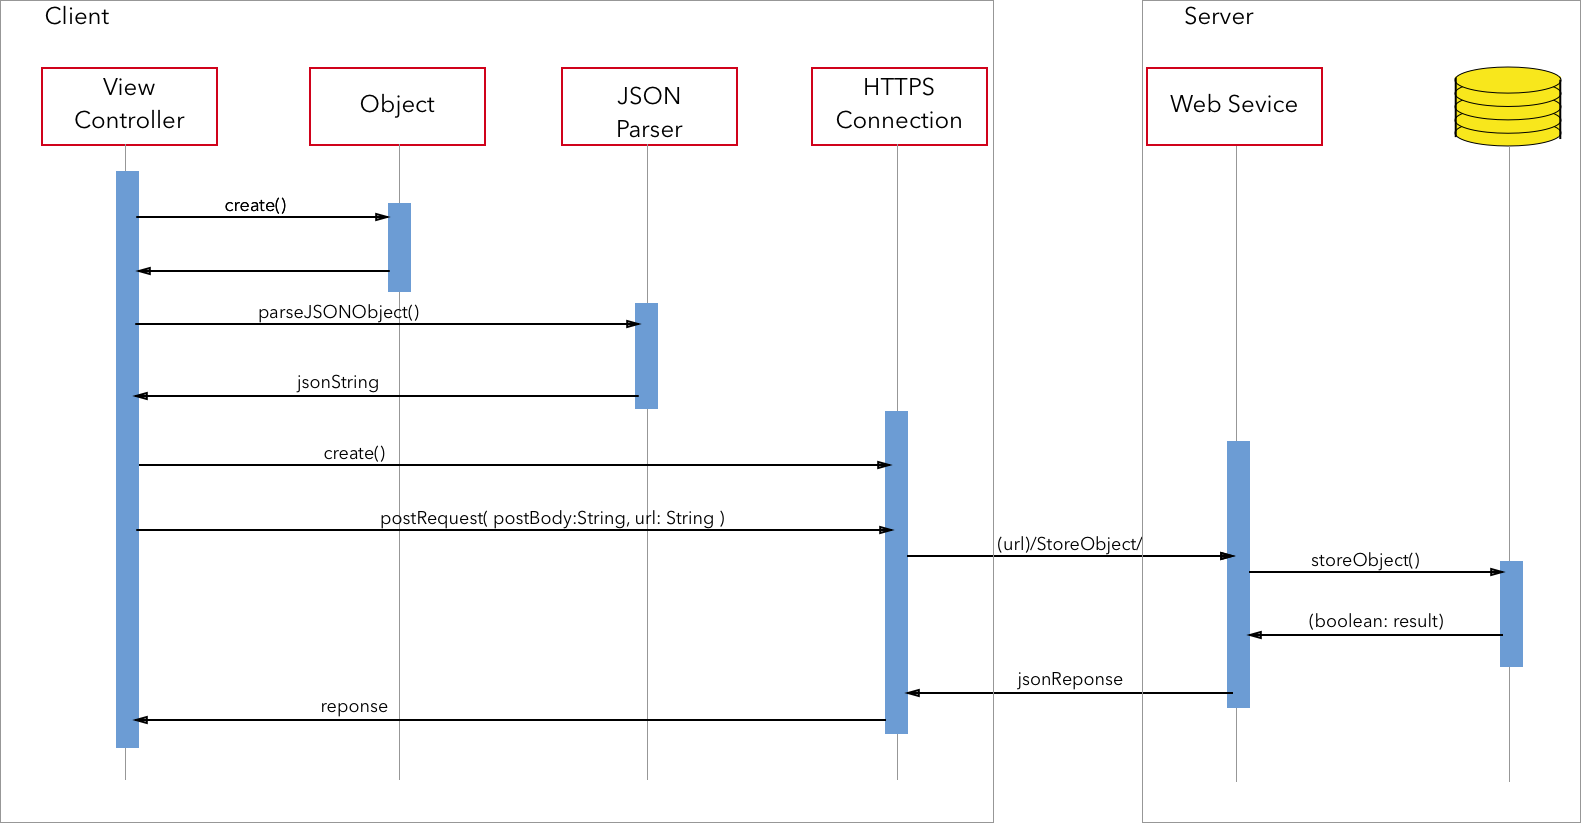
\includegraphics[width=100mm]{images/services/storage_sequence_current}
    \label{fig:storage_old}
\end{figure}


\begin{figure}[!h]
    \caption{Storage Sequence New}
    \centering
    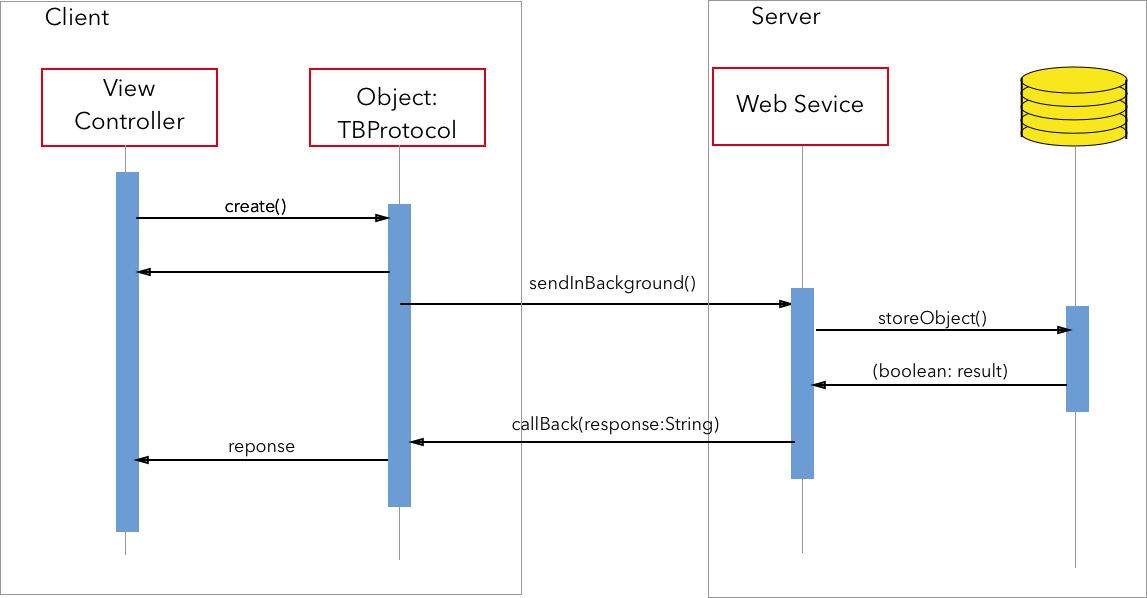
\includegraphics[width=100mm]{images/services/storage_sequence}
    \label{fig:storage_new}
\end{figure}

The two Figures \ref{fig:storage_old} and \ref{fig:storage_new} show the difference between developing the standard way, with the developing having to create a JSON parser and then set-up an HTTPS connection to send it to the server in Figure \ref{fig:storage_old} . The new way in Figure \ref{fig:storage_new} using the project’s storage protocol involves the developer only having to create the object, then using the functionality of the object to send it to the server.

\subsubsection{Apple Push Notifications (APNs)}

\paragraph{Server}
The APNs uses JSON Web Tokens (JWT) to authenticate the credentials for the connection. This uses two keys, public and private where Apple where keeps the public and the private which is a .p8 file is used from the sender. In this system, the private key needs to be upload to the directory in which the web server reads from.  Several steps are required to accomplish this. The developers must have a developer account with Apple, then in the developer console, the .p8 key can be created and downloaded. After the web server test project required accessing that file to send notifications. The DIT-Timetable app was used to verify receiving the push notifications.

\begin{figure}[!h]
    \caption{APNs \cite{apns}}
    \centering
    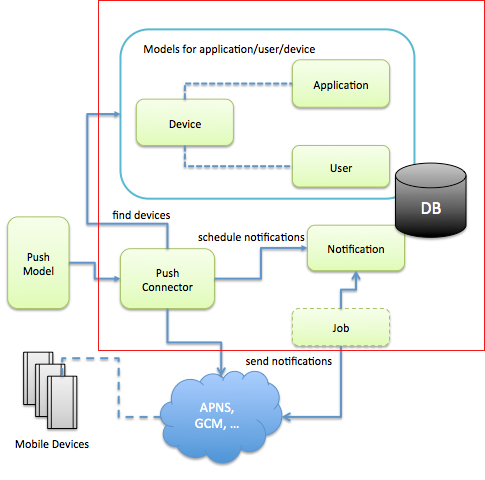
\includegraphics[width=75mm]{images/APNs}
    \label{fig:apns_overview}
\end{figure}

In Figure \ref{fig:apns_overview} represents the stages in which to send push notifications. Inside the red box is the server layer, where the .p8 file is located, the push model is where the messages originate. The notifications go through Apple's sandbox APNs, then on to the mobile devices.

\paragraph{Client}

The APNs tool was implemented in the library, for which the developer can use the notification object to send a request to the server, which in turn sends the notifications. The notification's object requires a list of values to be set for the notifications to work.

\begin{itemize}
  \item Universally Unique Identifiers
  - the target's device unique id to which apple will the notification.
  \item Message
  - message which the source wants to send to the target.
  \item Badge Number
  - each notification can be assigned a number, which displays on the app icon.
  \item Title
  - the title of the notification, usually the app name.
\end{itemize}

The following table \ref{table:mob_apns} demonstrates notification library to send notifications.

\begin{table}[!h]
\centering
\caption{APNS Library}
\label{table:mob_apns}
\begin{tabular}{|c|c|c|c|}
\hline
\rowcolor{green!20}
Library Method                    & Description                        & Parameters    & Result              \\ 
\hline
TBNotification.sendNotification();        & \makecell{Sends notifications\\ object to server} &  None & Successful/ Error   \\ 
\hline
\end{tabular}%
\end{table}

Figure \ref{table:apns} shows how to use the API requests outside of the library.

\begin{table}[!h]
\centering
\caption{Analytics API Requests}
\label{table:apns}
\begin{tabular}{|l|l|l|l|}
\hline
\rowcolor{green!20}
API Call                        & HTTP Method & Description                    & Parameters   \\ \hline
/\{appKey\}/notification & POST        & send notification object       & JSON Object  \\ \hline
/\{appKey\}/storage/TBNotification & GET         & Retrieves all notification objects & JSON Objects \\ \hline
\end{tabular}
\end{table}


\subsubsection{Analytics}

The first part for the analytic developed was the creation of the Perfect web-server which excepted POST requests. A playground application was developed with the lines of code in Listing \ref{lst:playground} to aid with HTTP requests. This class gathers some information before sending the request including, time-stamp, build version, OS version, device make and model. For the purposes of testing this service, the data was hard-coded in separate function, that in turn would be reading from plist file. Some of methods and the parameters are included in the following Table \ref{table:mob_analytics} which shows how to use the library to send analytics. The server stores the analytic objects in the database corresponding to the application, this is done using the appKey which is sent up in the API request.

\begin{table}[!h]
\centering
\caption{Analytics Library}
\label{table:mob_analytics}
\begin{tabular}{|c|c|c|c|}
\hline
\rowcolor{green!20}
Library Method                    & Description                        & Parameters    & Result              \\ 
\hline
TBAnalytics.sendOpenApp();        & \makecell{Sends up object\\ with open app type} &   \makecell{view: UIView , \\ method: String? = \#function \\ , file: String? = \#file } & Successful/ Error   \\ 
\hline
TBAnayltics.send();               & \makecell{Send up object \\ with type as option} &  \makecell{ app: UIResponder, \\ type: SendType \\ , method: String? = \#function ,  \\ file: String? = \#file } & Successful/ Error   \\ 
\hline
 \makecell{ TBAnayltics \\.getAllInBackground(); } & \makecell{Retrieves all \\ TBAnayltic objects }   & NONE        & Array of TBAnayltics \\ 
\hline
\end{tabular}%
\end{table}

Figure \ref{table:analytics} shows how to use the API requests outside of the library.

\begin{table}[!h]
\centering
\caption{Analytics API Requests}
\label{table:analytics}
\begin{tabular}{|l|l|l|l|}
\hline
\rowcolor{green!20}
API Call                        & HTTP Method & Description                    & Parameters   \\ \hline
/\{appKey\}/storage/TBAnalytics & POST        & Uploads analytics object       & JSON Object  \\ \hline
/\{appKey\}/storage/TBAnalytics & GET         & Retrieves all analytic objects & JSON Objects \\ \hline
\end{tabular}
\end{table}


\subsubsection{Remote Configuration} \label{dev:sub_rc}

The remote configuration service development is broken up into four sections.

\begin{itemize}
  \item JSON files 
  - where the configuration objects will reside on the phone
  \item JSON file manager
  - how the retrieving of the values
  \item Objects configuration
  - how each interface object can be configured
  \item Remote updating
  - updating the configuration file
\end{itemize}

This section will discuss the first three, the remote updating will be explained in dashboard development section.

\paragraph{JSON files}

The first part was the development the JSON file layout. The design chapter already discussed the design of the remote configuration, where each class object will contain the objects relating to that class, and subsequently, the objects properties will be on the object. To help with this, the storage protocol \textit{TBJSONSerializable} was used to be able to parse the objects into JSON string. In Listing \ref{fig:rc-cd} illustrates the class diagram for the complete remote configuration structure.

\begin{figure}[!h]
    \caption{Remote Config Class Diagram}
    \centering
    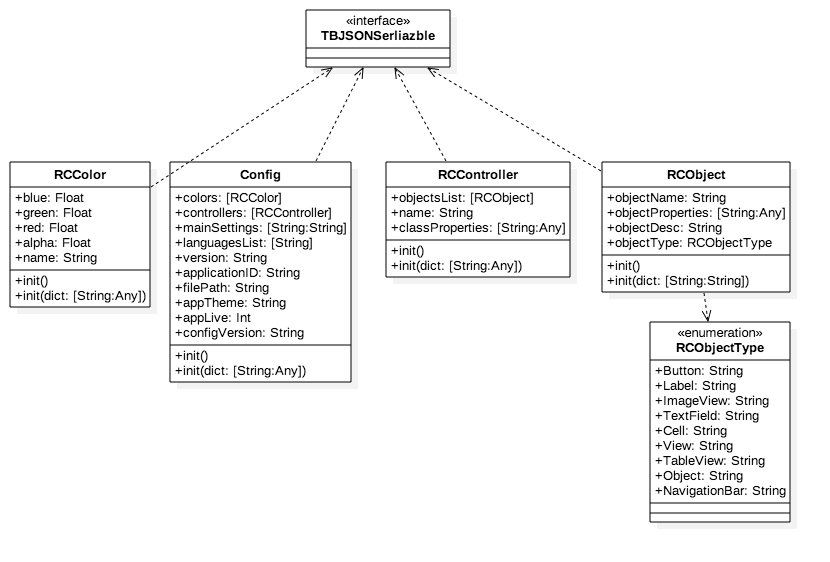
\includegraphics[width=150mm]{images/classdiagrams/config}
    \label{fig:rc-cd}
\end{figure}

% possibly add some code references to show the class variable names.

In Figure \ref{fig:rc-cd}, the remote configuration structure consists of 5 classes. The very first class of the structure is the Config class and is where all the other class objects will be located. The \textit{Config} class holds many properties, the first being the colours value, where all colours used in the application will be stored. The \textit{RCColour} object contains the red, green and blue (RGB) values along with alpha and the name of each colour. This name will be used in the properties value of each object, for example, the background colour. Next is controllers of type \textit{RCController}, these are the main classes or commonly known as \textit{ViewControllers} in the mobile app.

Moving on to the \textit{RCController} class, the properties include the name of that class which is the same variable name in app code The class properties, for example, if that class is of type \textit{UIViewController}, that class will contain \textit{backgroundColor} property, etc. The last major property is \textit{objectList} of type \textit{RCObject}. This is where all objects such as labels, text fields, tables, etc. will be stored. The \textit{RCObject} class contains the name of the object, along with its properties, these are what are provided by the framework when developing an app. The object type property is a type of enumeration which will contain what base class name is, for example, \textit{UILabel}. The reason for this will be explained later in the dashboard development section.

Back to the \textit{Config }class, the main setting variable is key value pairs that hold the primary data such as URLs values; these are stored at this level to speed up retrieval. The language list is as the name states contain the list of translation languages that the end user can change. This will be explained later in the language service section.

% \lstinputlisting[label={lst:config},language=Swift, caption=Configuration Structure]{development/code/config.m}

% In listing \ref{lst:config} lines 3 - 6 inclusive, holds the configuration objects for the applications. The colours objects is where all colours used in the app will be, this was placed here to speed up retrieval of each colour. The controllers objects is an array of view classes used within the app, then subsequently not shown are the objects within each class, and the properties relating to each object. The mainSettings variable on the same line of colours was placed here to speed up the retrieval of any import key values in the app such as URL. Last the languages list holds the list of languages available to the application. The languages part is based on the same as configuration files.

% Lines 8 - 13 are to distinguishes this configuration file with another, so when an update of configuration is done, then the application call tell if it has the latest or needs to download. This is to stop re-downloading the same file over and over again. The following listing \ref{table:json_manager} shows the library methods which to use the remote configuration files.

\paragraph{JSON file manager}

Table \ref{table:json_manager} illustrates some of the main functions available in the library. The function performs a read on the JSON files based on parameters being passed in and returns a value to be used. This functions can be utilised by the developer throughout the mobile app and also used in next section for the objects configurations.

\begin{table}[!h]
\centering
\caption{JSON file manager}
\label{table:json_manager}
\begin{tabular}{|c|c|c|c|}
\hline
\rowcolor{green!20}
Library Method                    & Description                        & Parameters    & Result              \\ 
\hline
RCConfigManager.getColor();        & \makecell{retrieval of\\ colour} &   \makecell{ name: String, defaultColor: UIColor } & UIColor   \\ 
\hline
 \makecell{RCConfigManager\\.getTranslation(); }  & \makecell{retrieval of\\ translation value} &  \makecell{  name: String, defaultName: String  } & String  \\ 
\hline
\makecell{ RCConfigManager \\.getMainSetting(); } & \makecell{retrieves main\\ setting value  }   & \makecell{  name: String, defaultName: String } & String \\ 
\makecell{ RCConfigManager \\.getObjectProperties(); } & \makecell{retrieves object\\ properties  }   & \makecell{  className: String, objectName: String } & [String:AnyObject] \\ 
\hline
\makecell{ RCConfigManager \\.getConfigVersion(); } & \makecell{gets latest version\\ of config file  }   & None & call back method \\ 
\hline
\makecell{ RCConfigManager \\.getConfigThemeVersion(); } & \makecell{gets latest version\\ of config theme file  }   & None & call back method \\ 
\hline
\end{tabular}
\end{table}


\paragraph{Objects configuration}

Object configurations involve how to get the object properties and update the user interface (UI) object. In the design chapter, it was discussed that a protocol along with protocol extension would be used for each UI object. A separate protocol for each UI object will be developed.  A protocol is first defined, then an extension to that protocol to add the implementation. A snippet example of \textit{UILabel} object is in the following Listing \ref{lst:protocol}

The extension \textit{LabelLoad} is restricted for classes with type \textit{UILabel}, and the developer has two methods it can use to implement. Inside the setup function, the object properties are retrieved from the JSON files in line 12 and then set to the corresponding property value in lines 15 and 18. The implementation chapter demonstrates
 how this labelling protocol can be used.

\lstinputlisting[label={lst:protocol},language=Swift, caption=UILabel Protocol]{development/code/protocol.m}

\subsubsection{A/B Testing} \label{dev:sub_ab}

A/B Testing utilises two other services, remote configuration and Analytics. The JSON files can tell what version of configuration is being used, so when an analytic object is sent up, the version is included. The server, however, needs some development to handle A/B Testing. The dashboard explained later is used to set what mobile applications and versions will be involved in an A/B Testing. When a request comes into the web server for the configuration file, a check on the A/B Testing list is done to check whether that app version exists as seen in Figure \ref{fig:abtesting-cd}. 

\begin{figure}[!h]
    \caption{A/B Testing Class Diagram}
    \centering
    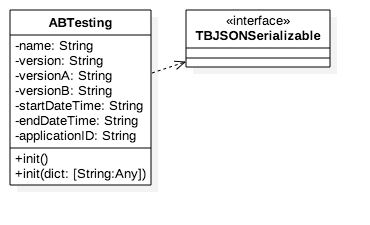
\includegraphics[width=100mm]{images/classdiagrams/ABTesting}
    \label{fig:abtesting-cd}
\end{figure}

The class diagram comprises of the \textit{ABTesting} table along with the protocol TBJSONSerializable mentioned earlier. The table properties include the name of the testing, the application id and app version for that testing. The \textit{versionA} and \textit{versionB} are the two different configuration files and the dates for which the testing is in place.

To develop this service on the server, a singleton class (which is a class that has only one instance in the life of an app) \textit{RemoteConfig} is used. When the server starts up, the singleton class is initialized with a current request number of zero. With each request, the count increases, and using this value can depend on what version of the configuration file that users get. The web servers section illustrates the singleton using a sequence diagram later.

% \subsubsection{Live Database}

\subsubsection{Exception catching} \label{dev:sub_exception}

The design chapter explained there are two types of exception catching, uncaught and caught exceptions. Both types need to develop in different ways, as one would potentially crash the app, so would not able to send a POST request to the server. Not only are there two types of exceptions, but each exception has a different level, so when the developer views the dashboard, they can set a priority. The various levels are Fatal, Error, Warning, Info and Debug.

The exception was developed using a singleton class to that all exceptions can be sent through. When the app opens, the exception objects gets initialized which includes setting the \textit{NSSetUncaughtExceptionHandler()} which is Apple’s uncaught exception handler, where the parameter is an internal function name which looks after catching the exception. The following Figure \ref{fig:exception-cd} illustrates the exception class. The tags properties hold values relating to the device type, the OS running, etc., the rest of the values are about the exception values.

\begin{figure}[!h]
    \caption{Exception Class Diagram}
    \centering
    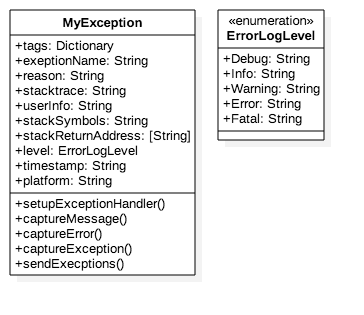
\includegraphics[width=100mm]{images/classdiagrams/Exception}
    \label{fig:exception-cd}
\end{figure}

\paragraph{Uncaught exceptions}

Uncaught exceptions make the app crashes, so between the time crash happens and the app closes which is a small window, the exception has to be dealt with. Using the \textit{NSSetUncaughtExceptionHandler()} with the parameter of the function, that function is not allowed to make outside calls, which include HTTP request and function calls. So the exception is stored in \textit{UserDefaults} which is a built-in the data dictionary that stores a few user settings for as long as the app is installed. When the user opens application again, the exception singleton class gets instantiated, and it does a check if any exceptions exist in \textit{UserDefaults}, and then an HTTP post sends the exception to the server. 

The Listing \ref{lst:exception} shows the code required to catch uncaught exceptions. On line 21, Apple’s function takes a parameter which has to be an internal function name. The internal function called \textit{exceptionHandler} takes a parameter of type \textit{NSExeception}, which contains values such as the reason and the call stack. As this function can not make outside requests, its stores the values in UserDefaults storage. When the application opens again, the function on line 2 gets called which reads the stored values and sends them to the server.

\lstinputlisting[label={lst:exception},language=Swift, caption=Exception handling]{development/code/execption.m}

\paragraph{Caught exceptions}

Extra functionality was added to using the same class as above with uncaught exceptions to enable developers to send these exceptions to the server. As the class is a singleton and gets initialized when the application opens, the \textit{sharedClient} function can be used to return the instance of that object, then use the functions available to send the caught exceptions. Some of these are shown in Table \ref{table:exceptions}

\begin{table}[!h]
\centering
\caption{Caught Exceptions}
\label{table:exceptions}    
\begin{tabular}{|c|l|l|l|}
\hline
\rowcolor{green!20}
\multicolumn{1}{|l|}{Library Method}                             & Description                                                                                            & \multicolumn{1}{l|}{Parameters}                                                                                                        & Result            \\ \hline
\begin{tabular}[c]{@{}c@{}}MyException.\\ sharedClient.\\ captureMessage();\end{tabular} & \begin{tabular}[c]{@{}l@{}}Captures the info message \\ and sends to the server\end{tabular}           & \begin{tabular}[c]{@{}c@{}}message : String,\\ method: String? = \#function, \\ file: String? = \#file, line: Int = \#line\end{tabular}                        & Successful/ Error \\ \hline
\begin{tabular}[c]{@{}c@{}}MyException.\\ sharedClient.\\ captureMessage();\end{tabular} & \begin{tabular}[c]{@{}l@{}}Captures the message\\  along with error level\\ to the server\end{tabular} & \begin{tabular}[c]{@{}c@{}}message: String, level: ErrorLogLevel, \\ method: String? = \#function , \\ file: String? = \#file, line: Int = \#line\end{tabular} & Successful/ Error \\ \hline
\begin{tabular}[c]{@{}c@{}}MyException.\\ sharedClient.\\ captureError();\end{tabular}   & \begin{tabular}[c]{@{}l@{}}Captures the error \\ and sends to the server\end{tabular}                  & \begin{tabular}[c]{@{}c@{}}error : NSError, method: String? = \#function,\\  file: String? = \#file, line: Int = \#line\end{tabular}                           & Successful/ Error \\ \hline
\end{tabular}
\end{table}


\section{Integrate into Live App} \label{dev:integration}

For some parts of the project, an already developed and published app called DIT-Timetable was used to add in the services, to test if Apple would allow it through. The services include remote configuration and language choice. Due to Apple's strict guidelines, the remote configuration was developed into the DIT-Timetable app into different phases, then each stage had a build and published.

\subsubsection{Phase 1}
This phase included just the basic remote configuration, with the capability of updating text such as page title, and label values. Apple did approve this phase meaning that the app using the iPad prototyping app can be updated.

\subsubsection{Phase 2}

Phase 2 gave the ability to adjust user interface values such as text colour, text size and user interaction enabling/disabling. This also has been approved by Apple giving it a go ahead to be completely integrated into the project.

\section{Web-server} \label{dev:webserver}

The web server developed was split up into two sections; the development of the web-server using the framework Perfect with setting up the server and creating the installation file which will install all the required dependency packages.

\subsubsection{Development} \label{dev:ws_dev}

To start developing the server, Perfect provides a basic template with just the structure to start off with, found at \ur{https://github.com/PerfectlySoft/PerfectTemplate}. A new directory was created, then running the command: \textit{git clone \url{https://github.com/PerfectlySoft/PerfectTemplate.git}}. One the template was download, running the following command would create the Xcode project: \textit{swift package generate-xcodeproj}. 

A package manager tool is for managing the distribution of Swift code. It automates the process of downloading, compiling and linking dependencies. The package consists of the source files and a manifest file called \textit{package.swift}. It defines the packages names and contents using the \textit{PackageDescription}. \cite{swift_manager} The package.swift file required updating with the required packages such as MongoDB and Notifications etc, then running the command \textit{sudo swift build} inside the project directory retrieved all the packages that were included in the package.swift file. The project structure contains sources and packages directories, the packages are which was already downloaded and the sources where the web-server files are placed. 

The web-server starts off with the \textit{main.swift} which includes the creation the HTTP server, and adding routes and setting the port number, then starting the server. The routes are where each REST request goes, so for example if request /user then the route will go to the user class. An example of the routes is shown in listing \ref{lst:routes}. This example is the routes for the database, retrieving and sending object. The function is called from the \textit{main.swift} file, which returns all the routes for the database handler class. The handler parameter is the method name in the same class for which implementation is done depending on the route.

\lstinputlisting[label={lst:routes},language=Swift, caption=Routes]{development/code/routes.m}
% Instead of creating a new app for each service as already mentioned before which does not follow the programming principle "Only write it once".

The web-server deliverable consists of a collection of apps. These apps is a web application that does something e.g. database of records. The design chapter under web-server section \ref{d-web_server} discussed the overview structure, and what web apps are to be developed. This section will discuss the development of each web app and what functionality is required.

\paragraph{Database}

\begin{figure}[!h]
    \caption{Database Sequence Diagram}
    \centering
    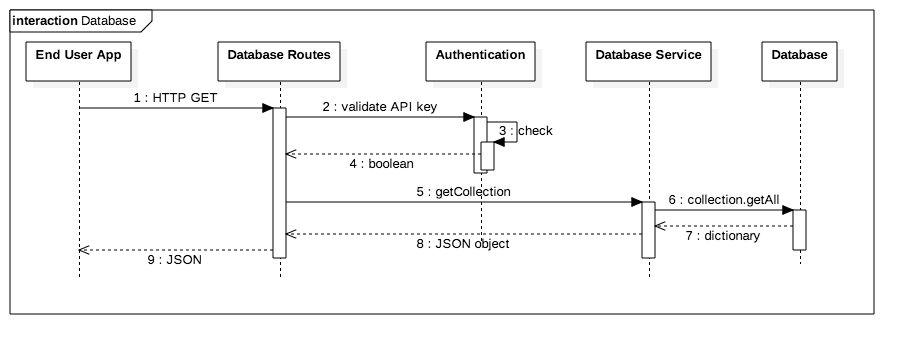
\includegraphics[width=150mm]{images/sequence/Database}
    \label{fig:database-seq}
\end{figure} 

The database app consists of four layers; the routes, authentication, service and the database as can be seen in figure \ref{fig:database-seq} This allows the app to be loosely coupled meaning the database type can be changed without having to change the other layers. The objective of this app is to perform the four basic functions of persistent storage; create, read, update and delete (CRUD). So the first four routes were developed, and the collection name was required to be passed as a parameter as this is a generic app, the collection names would not be known until the developer creates them. This is show in Table \ref{tb:db-routes}, where the app key is also passed to be authenticated. 

\begin{table}[!h]
\centering
\caption{Database routes}
\label{tb:db-routes}
\begin{tabular}{|l|l|}
\hline
\rowcolor{green!20}
Route                                  & HTTP Method \\ \hline
/api/\{appkey\}/storage/\{collection\} & GET         \\ \hline
/api/\{appkey\}/storage/\{collection\} & POST        \\ \hline
/api/\{appkey\}/storage/\{collection\} & DELETE      \\ \hline
\end{tabular}
\end{table}

The database service layer function is called depending on the route; the service layer will then communicate with the database class to perform the task. The database class performs five steps for each of the CRUD operations;

\begin{itemize}
  \item Open client connection
  - the connection being the Uniform Resource Identifier (URI) : "mongodb://localhost:27017" 
  \item Database 
  - connect to correct database depending on the application
  \item Collection
  - get the collection from the collection name which is passed in
  \item Find
  - run the query and pass in anywhere clauses if required
  \item Close
  - close the collection, then database and finally the client
\end{itemize}

Once these steps have finished, the function returns the search records, which in returns parses the records into JSON form to be sent back in the response object. After the four basic functions were completed, extra functionality was added to be able to pass query dictionary from the mobile application for example \textit{{``name``:``tim``}} which will return all records where name key contains values equal to \textit{tim}. This was developed by creating another route along with function which accepts the dictionary query and then includes this in the find function. Next, the routes had to be added for the dashboard to make requests, for example, to retrieve all databases and in turn all collections relating to each database. This is used in the database page called Storage already discussed above.

\paragraph{File}

\begin{figure}[!h]
    \caption{File Sequence Diagram}
    \centering
    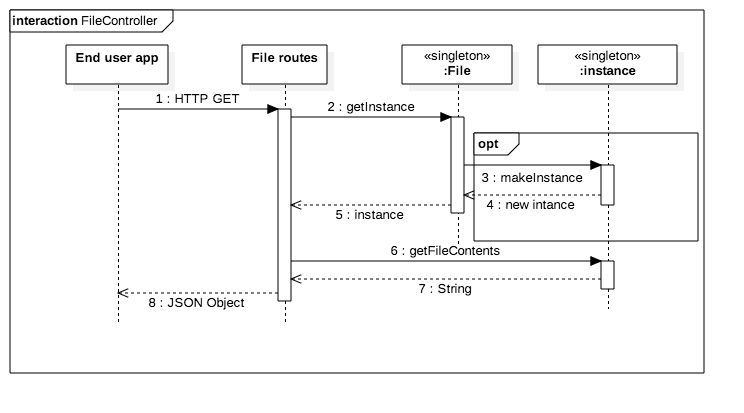
\includegraphics[width=150mm]{images/sequence/FileController}
    \label{fig:file-seq}
\end{figure}

This web app provides two purposes, one for uploading of files of any type and storing from the mobile app, as well as other web apps such as remote config discussed next to retrieved a stored file. The Figure \ref{fig:file-seq} illustrates the steps required to manage files. This web app class using a singleton pattern. The difference between singleton class and regular class is that only one instance is made upon run time, this helps controller file writing so that two instances are not trying to write to the same file at the same time.

\begin{table}[!h]
\centering
\caption{File Handler Routes}
\label{tb:file-routes}
\begin{tabular}{|l|l|}
\hline
\rowcolor{green!20}
Route                                        & HTTP Method \\ \hline
/api/\{appkey\}/upload/\{directory\}/          & POST        \\ \hline
/api/\{appkey\}/upload/\{filepath\}/ & GET         \\ \hline
\end{tabular}
\end{table}


The routes to handler send and retrieving files as shown in Table \ref{tb:file-routes}. The post route sends up the files to a particular directory path which is set from the client application side, as well as the file names. After the file handler has successfully saved the files in the specified directory, the file controller class calls the database service class and inserts the file's meta-data that has been upload as history records.

This structure for the file web app allows the access from other apps such as the remote configuration and language to access the singleton class. Inside the class, there are a collection of functionalities required such as setting the working directory. This is another reason for using the singleton pattern, as every time the working directory is called, it creates a new directory which would cause files to be lost in a multitude of sub-folders. The instantiation of the file class happens when the server starts up in the \textit{main.swift} file, thus given all over apps access to one working directory.

Extra functionality was required if a file path does not exist, then the directories need to be created. An example of this would be if file path were \textit{`/files/cars/image1.PNG`}, and the cars directory currently did not exists then steps is required to ensure the file location was correct.

\begin{enumerate}
  \item check if the path exists
  - if true then overwrite 
  \item if path does not exit
  - get directory path from file path string = \textit{`/files/cars/`}
  \item create file path
  \item save file to location
\end{enumerate}


\paragraph{Remote Configuration}

\begin{figure}[!h]
    \caption{Remote Config Sequence Diagram}
    \centering
    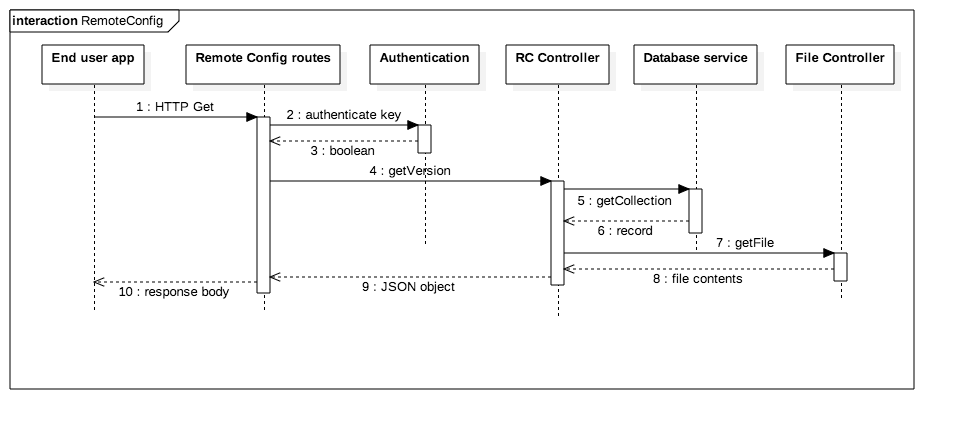
\includegraphics[width=150mm]{images/sequence/RemoteConfig}
    \label{fig:rc-seq}
\end{figure}

\begin{table}[!h]
\centering
\caption{Remote Config Routes}
\label{tb:rc-routes}
\begin{tabular}{|l|l|}
\hline
\rowcolor{green!20}
Route                                        & HTTP Method \\ \hline
/api/\{appkey\}/remote                       & POST        \\ \hline
/api/\{appkey\}/remote/\{version\}           & GET         \\ \hline
/api/\{appkey\}/remote/\{version\}/\{theme\} & GET         \\ \hline
\end{tabular}
\end{table}

As illustrated in Figure \ref{fig:rc-seq} operations are required to retrieve the configuration file contents. The HTTP GET request with the right route seen in table 5.11 is made, then the app key is again authenticated if passed the \textit{RCController} class is called to get a version file. The \textit{RCController} makes a call to the database service class for the collection of remote configuration along with the query of the app version. The record is returned to a file path; then file controller class is called to return the contents of the file.

\paragraph{A/B Testing}

\begin{figure}[!h]
    \caption{A/B Testing Sequence Diagram}
    \centering
    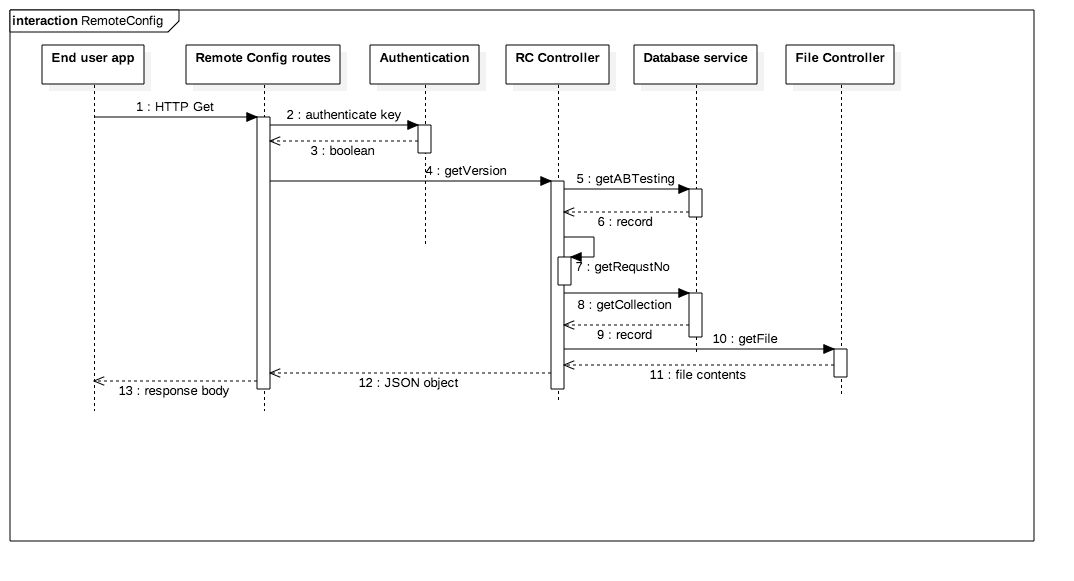
\includegraphics[width=150mm]{images/sequence/ABTesting}
    \label{fig:ab-seq}
\end{figure} 

The A/B Testing service discussed in the services section above requires extra functionality, this is illustrated in Figure  \ref{fig:ab-seq}. An additional query to the database service was added to \textit{RCController} class to get the records if any of A/B Testing. The A/B Testing records contain the application version which is queried from the version passed in, if the return contains a record, then a request to itself is made to get the request number. This request number is the total number of requests made modular 2, so depending on the number depends on what version A or B is returned to the response body. The \textit{RCController} class is a singleton, meaning it only has one instance, and this was used to store the request no, instead of writing to a text file which would cause performance issues.

\paragraph{Authentication}

\begin{figure}[!h]
    \caption{Authentication Sequence Diagram}
    \centering
    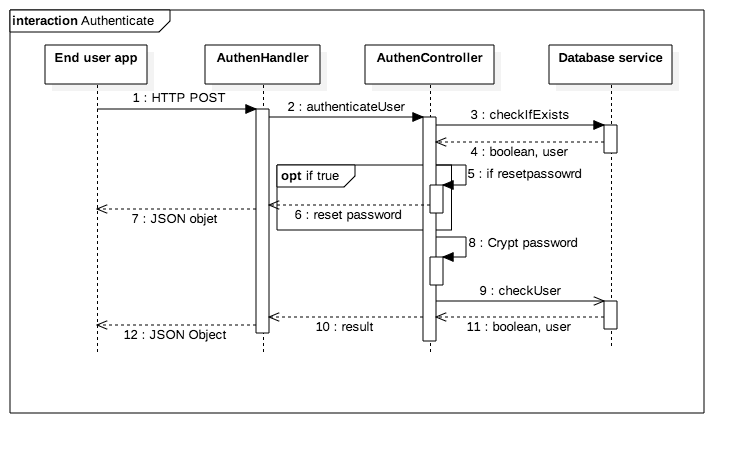
\includegraphics[width=150mm]{images/sequence/Authenticate}
    \label{fig:authenticate-seq}
\end{figure}

Figure \ref{fig:authenticate-seq} illustrates the required steps to authenticate a user when signing in. The HTTP request method is POST to keep both username and password out of URL parameters for security purposes. The authentication handler class which handles the routes passes the values to the authentication controller class which performs four steps. The first step is to ensure the user exist using the username, next it does a check if the password reset field has been set to 1 meaning the administrator has authorised this account for the password to be changed. If the result is true, the message is sent back to the client app for the developer to allow the user to change the password. If the reset password flag has not been sent, then the password is first encrypted using the salt value used when registering.

The salt value is stored in a separate table for security reasons and is a one-way hashing function. The primary reason for using salt is to defend against dictionary attacks, historically a password would have been stored in plain-text, but over time additional steps were in placed to safeguard the password and one these ways is called Salting. After the password has been salted, then the query can be run by passing the username and hashed password, and if there returns one record, then the client app is sent an authentication message.

\paragraph{System}

The system handler and controller class are for the dashboard status view, the data for the four pie charts being CPU, memory and storage usage. This data is retrieved by running Linux commands from the server. The overview structure of this web app includes the system handler which only handles a get request for retrieving all the required data. The system controller class contains functions for each pie chart data, which is shown in Table \ref{tb:system} along with the command and output. 

\begin{table}[!h]
\centering
\caption{My caption}
\label{tb:system}
\begin{tabular}{|l|l|l|}
\hline
\rowcolor{green!20}
Function name    & Linux command & Values retrieved       \\ \hline
getCPUUsuage()     & top -bn1      & user, system, idle     \\ \hline
getMemoryUsuage()  & free -m       & total, used, available \\ \hline
getStorageUsuage() & df -h         & size, used, available  \\ \hline
\end{tabular}
\end{table}

The CPU usage is retrieved by running the \textit{top} which displays all Linux tasks; the \textit{-b} option puts the top in batch mode operation. The batch mode stops top from accepting any input until top has exited.The \textit{n1} is the number of iterations or frames to be run before ending, in this case, one. The output is then parsed into a dictionary for user, system and idle. 
The \textit{free} command displays the amount of free and used memory in the system. The \textit{-m} option displays the output in MBs format. The result creates a list of columns, and the string is parsed and the total, used, and free values are appended to the dictionary. 
The \textit{df} command gets a report of the disk space usage, and using the \textit{-h} options returns the result in human readable format, e.g., 1K, 512M 2GB. After the three commands are run, the result is sent back to the response body parsed in JSON format to be read by the status view class.

\paragraph{Backup}

\begin{figure}[!h]
    \caption{Backup Sequence Diagram}
    \centering
    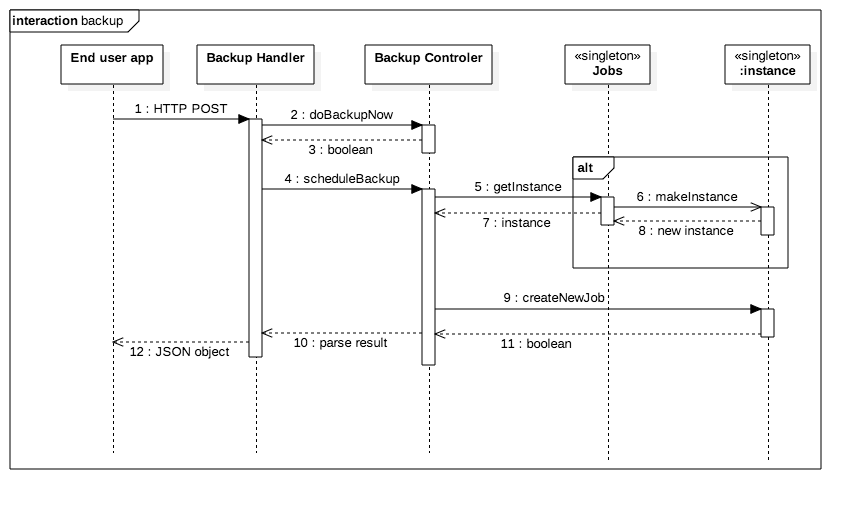
\includegraphics[width=150mm]{images/sequence/backup}
    \label{fig:backup-s}
\end{figure}

The backup feature discussed in the dashboard sections requires the web-server to do a complete backup of all database collections and files to a remote or local location. The sequence diagram in Figure \ref{fig:backup-s} illustrates the steps required to accomplish this. The sequence diagrams display two types of requests if a backup is required to be done now or scheduled for a later time. The first is quite simple with the request coming in and passed to the backup controller class, and performs the required steps to accomplish the backup will be discussed after.

First, scheduling a backup requires a few more steps, the Jobs class is a singleton which keeps an instance of the \textit{CronJob} class. \textit{CronJobSwift} is a package provided by a developer called Ryan Collins with Github link \url{https://github.com/rymcol/SwiftCron-Example}. The \textit{CronJob} is on the same principle of Linux software utility called \textit{Cron} which is a time-based job scheduler. These jobs can repeatedly be run at certain times of the day, week, etc. to perform tasks in the background. The \textit{CronJob} class still requires to be kept running, and outside of the main.swift file to be updated with new jobs or cancelling jobs. The singleton pattern is used to maintain an instance of \textit{CronJob} running, and allow outside requests to update the jobs.

Back to the sequence diagram in Figure \ref{fig:backup-s}, the make instance method is only a fail-safe if the main file when the server starts up does not create the instance. When the instance is return back to the backup controller class, the job can be created and updated. All scheduled jobs are also stored in the database along with the job id, so that a request can be made to cancel a particular job.

Once the backup method has been called, a number of steps are required along with a package called Zip provided by Perfect. A Linux package is also required by running the following command \textit{apt-get install libminizip-dev"} The package for Swift zip can be found at the Github link \url{https://github.com/PerfectlySoft/Perfect-Zip}. The zip package will be used to put all the collections into one zipped folder so that it can store locally or remotely without potentially using up a lot of space.

\begin{enumerate}
  \item get list of database 
  \item get list of collections from each database
  \item stored the collections in a backup folder, sub-folded the collection name
  \item zip the backup folder with the current date
  \item move the zip folder to destination
  \item put history of the backup in the database
\end{enumerate}

\paragraph{Translations}

\begin{figure}[!h]
    \caption{Translation Sequence Diagram}
    \centering
    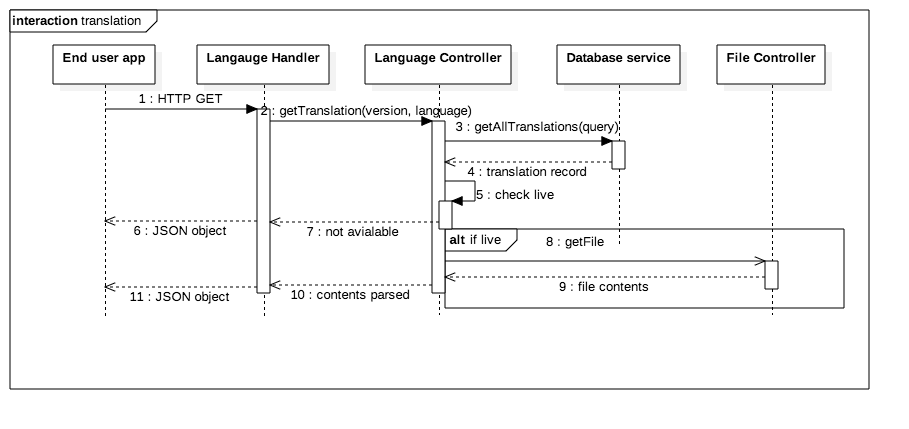
\includegraphics[width=150mm]{images/sequence/translation}
    \label{fig:translation-s}
\end{figure}

\begin{table}[!h]
\centering
\caption{Translation Routes}
\label{tb:translation-routes}
\begin{tabular}{|l|l|}
\hline
\rowcolor{green!20}
Route                                        & HTTP Method \\ \hline
/api/\{appkey\}/translation                  & POST        \\ \hline
/api/\{appkey\}/translation/\{language\}/\{version\}           & GET         \\ \hline
/api/\{appkey\}/translationVersion/\{language\}/\{langversion\} & GET         \\ \hline
\end{tabular}
\end{table}

The last web app to be developed is the translation, which handles posting and retrieving the correct translation version and language. The Table \ref{tb:translation-routes} illustrates the routes, where the first post request will send the translation object to both the database and file location. When a request is made for a translation file, an extra check is done to see if that version is available; this can be seen in the sequence diagram in Figure \ref{fig:translation-s}. This was discussed in the dashboard section, where the developer has the option of making a translation version live.

The translation and configuration files availability are put into the top object of any database GET request sent to the server. Listing \ref{lst:header_json} displays the header of an object when making a request, the current version and date of what is available on the server for both configuration and translation; then the application can make a request for the latest if required.

\lstinputlisting[label={lst:header_json}, caption=Header JSON]{development/code/header_json.m}

\paragraph{Testing environment}

The last part of the web server work was to develop a way to enable a testing environment. This was done using the library with each request being sent up to the server, included in the header was a value that is to set if the developer is in testing/debug mode. Then on the server side, a new database would be created automatically to handle storing the test data. The storage view in the dashboard has a new functionality where a replication of a database can be done with a naming convention of $<$database name$>$-Test. This provides the developer with live data without having the worry of destroying valuable users data.

\subsubsection{Deployment}

DigitalOcean was used as the server of choice and to create a virtual private server or as DigitalOcean calls them Droplets. After creating an account and going to the page to create a droplet, the first choice was of distribution. The project required Ubuntu 16.04, after which the droplet size was asked, as for this project the basic 512MB ram, 20GB SSD Disk and 1000 GB transfer package was chosen. The next option was what region the droplet will be located and decided to go with London being the closest. Step 5 was additional options where IPv6 was chosen, for Apples requires the server to contain both IPv4 and IPv6. Step 6 was setting up SSH keys, which was done, and the last step was to give the droplet a name for the dashboard purposes.

After the droplet had been created and to log in from the computer, the terminal was used with the following command: \textit{ssh root@$<$droplet IP address$>$}. Once the password had been entered, a prompt message asking to set up SSH keys and followed by entering YES. After logging in a list of steps to setup and install the required packages, while running these commands and checking they installed correctly, they were added to a script file which would be used to create the installation script.

\paragraph{Step 1}
The first step once logged in was to create a new user and password for security purposes. This was done by running the following commands in Listing \ref{lst:username}.

\lstinputlisting[label={lst:username}, language=Bash, caption=Setting user-name]{development/code/username.m}

\paragraph{Step 2}
Next, the server required to set the locale along with updating and upgrading.
\lstinputlisting[label={lst:init_server}, language=Bash, caption=Updating Server]{development/code/init_server.m}

\paragraph{Step 3}
To be able to run Perfect which is Swift based, Linux server requires the Swift package.
\lstinputlisting[label={lst:swift_install}, language=Bash, caption=Swift Installation]{development/code/swift_install.m}

\paragraph{Step 4}
The MongoDB database for persistent storage also required being installed.
\lstinputlisting[label={lst:mongo_install}, language=Bash, caption=MongoDB Installation]{development/code/mongo_install.m}

\paragraph{Step 5}
The supervisor is a service that can be installed to monitor and manage a program that is defined in the configuration file.The following Listing \ref{lst:supervisor} will set up GIT which is where the web-server will be installed, and then the supervisor will be installed and set-up.
\lstinputlisting[label={lst:supervisor}, language=Bash, caption=Supervisor]{development/code/supervisord.m}
At line 6 where the \textit{nano} command is run, the \textit{post-receive} file need to be updated to contain the project name.

\paragraph{Step 6}
Next, the web-server itself needs to pull from Github and then built. Once the build has been done, ownership for the folders needs to change. Then the built packages need to be moved into the running folder, which supervisor will pick up the server and start it.
\lstinputlisting[label={lst:web-server}, language=Bash, caption=Web-Server]{development/code/web-server.m}

\paragraph{Step 7}
For the web-server to be access from the outside the server, a server needs to be installed to route the requests to the web-server. Nginx is installed, and then some configurations need to be done. When running line 3 in Listing \ref{lst:server}, the port number needs to be updated to 8181 which is what the web-server runs on. Nginx will route traffic coming in at 80 and 443 which is HTTP and HTTPS to port 8181.
\lstinputlisting[label={lst:server}, language=Bash, caption=Nginx Server]{development/code/nginx_setup.m}

\section{Dashboard Development}

The dashboard was originally going to be created as an iPad app, but after some thought that not all mobile developers can be expected to own an iPad, the dashboard was developed as a Mac App. In the design chapter, the layout and design of the dashboard were discussed including what functionality will be provided to the developers.

\subsection{Project structure}

Xcode IDE was used to develop the dashboard interface with the help of libraries. These libraries included Cocoa(API) and Charts. Cocoa is Apple’s native object-oriented application programming interface (API) for their operating system macOS. The cocoa consists of the Foundation Kit, Application Kit and Core Data frameworks. It is responsible for the appearance of apps and their responsiveness to user actions. The Figure \ref{fig:cocoa} illustrates where the Cocoa frameworks reside. Charts is a third party framework provided by a developer called Daniel Cohen Gindi that can be found on Github. \cite{charts} 

Already discussed in the design chapter, Apple gives an extensive section on Human Interface Guidelines on which to follow when developing Mac applications. So following these guidelines will help develop an application that can be submitted to the Mac App store. The IDE that will be used as already stated is Xcode, inside Xcode, several views can be utilised. In the following sections, the two main areas which will be used are the Interface Builder and Code Editor views. The Interface Builder is where the storyboards can be edited. They are a user interface way of designing and developing the UI of an application, and the code editor view is what connects the UI view to the class files.

\begin{figure}[!h]
    \caption{Cocoa \cite{cocoa}}
    \centering
    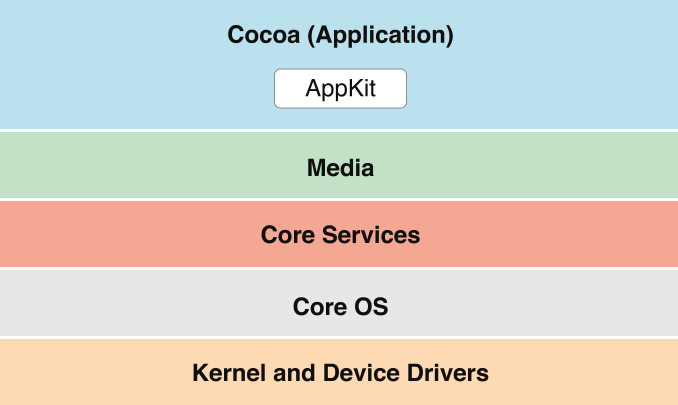
\includegraphics[width=75mm]{images/dashboard/cocoa}
    \label{fig:cocoa}
\end{figure}

\subsection{Dashboard Views}

\subsubsection{Login view}

\begin{figure}[!h]
    \caption{Log in class diagram}
    \centering
    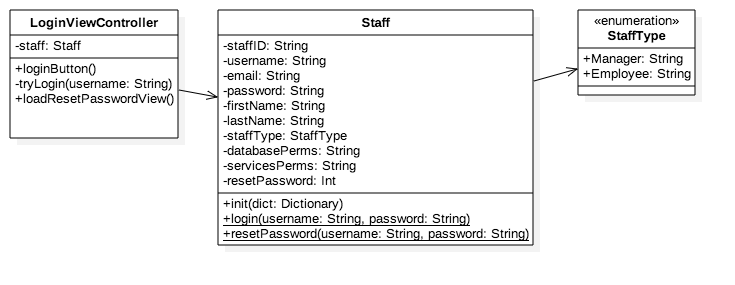
\includegraphics[width=150mm]{images/classdiagrams/Login}
    \label{fig:login_cd}
\end{figure}

Figure \ref{fig:login_cd} illustrates the class diagram of the main view controller for the login view, as well as the staff object that was used to authenticate the user. In Figure \ref{fig:log-in-view} illustrates the simple dashboard sign in view where the user gets verify their credentials. The view contains three input values which the user must put in, as the server can be deployed on any server, the user is asked to put in the IP or domain name where the server is located. The other two values are user-name and password, and then there is an option for the user to tick the remind me box, which keeps the user logged in. The Log-in button sends POST request to the server along with both values. A register button was decided against, as this is a restrictive application. The administrator once logged in can create new users explained later on.

\begin{figure}[!h]
    \caption{Login View}
    \centering
    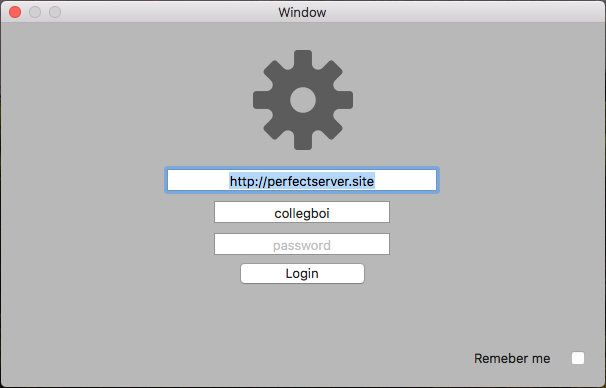
\includegraphics[width=75mm]{images/dashboard/login}
    \label{fig:log-in-view}
\end{figure}

\subsubsection{Status}

% change to include the menu view
\begin{figure}[!h]
    \caption{Status View}
    \centering
    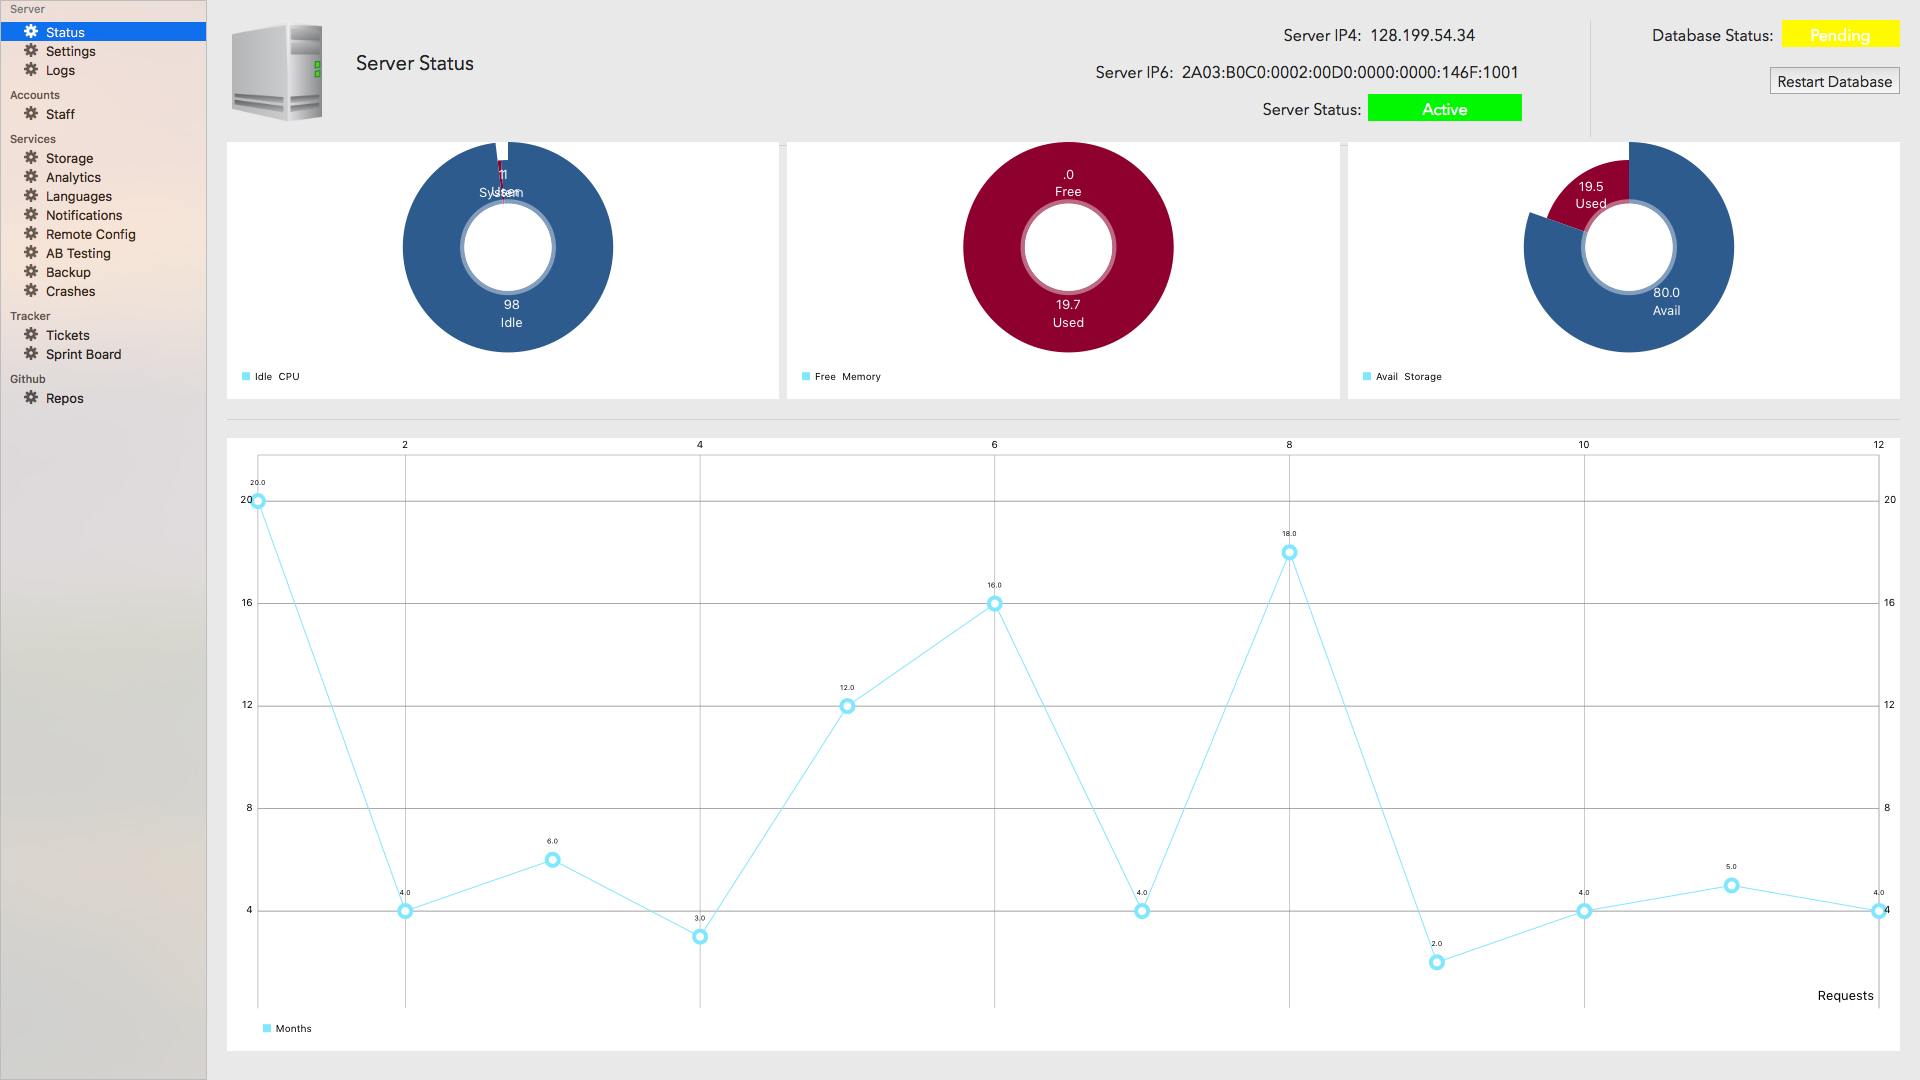
\includegraphics[width=100mm]{images/dashboard/status_view}
    \label{fig:status-view}
\end{figure}
% change to include the menu view

Before discussing the status view, the menu on the left will exist on view. The menu bar routes the user across the whole application. The bar contains grouped submenus to help clarify to the user what the view provides. The accounts section, for example, provides staff, so before clicking on this option, it is already known that it is staff accounts. This design is following Apple's guidelines on the mental model and consistency mentioned in the design chapter.

Figure \ref{fig:status-view} illustrates the server status view, it is the first page the user sees when entering the application. This view displays a number of graphs about the server. To help with displaying graphs, a framework was used called Charts, and listing \ref{lst:pie-chart} illustrates the code necessary to display a pie chart. In lines 1 to 4, the content of the chart is being populated. The values past are the sections within a pie chart, being the size of section and label name. The sections in line 9 are given their own color to help distinguish them.
% change to include the menu view
Starting from left to right with the pie charts, the first displays the current CPU usage, next storage usage and memory usage (last one). The line chart displays the history and current CPU usage. This gives the developer an general overview on what the physical sever doing. This can help decide whether or not to upgrade the system.
% change to include the menu view
\lstinputlisting[label={lst:pie-chart},language=Swift, caption=Pie Chart]{development/code/piechart.m}

The bottom line chart in figure \ref{fig:status-view}, displays the number of requests made over a period of time.

\subsubsection{Settings}

\begin{figure}[!h]
    \caption{Settings View}
    \centering
    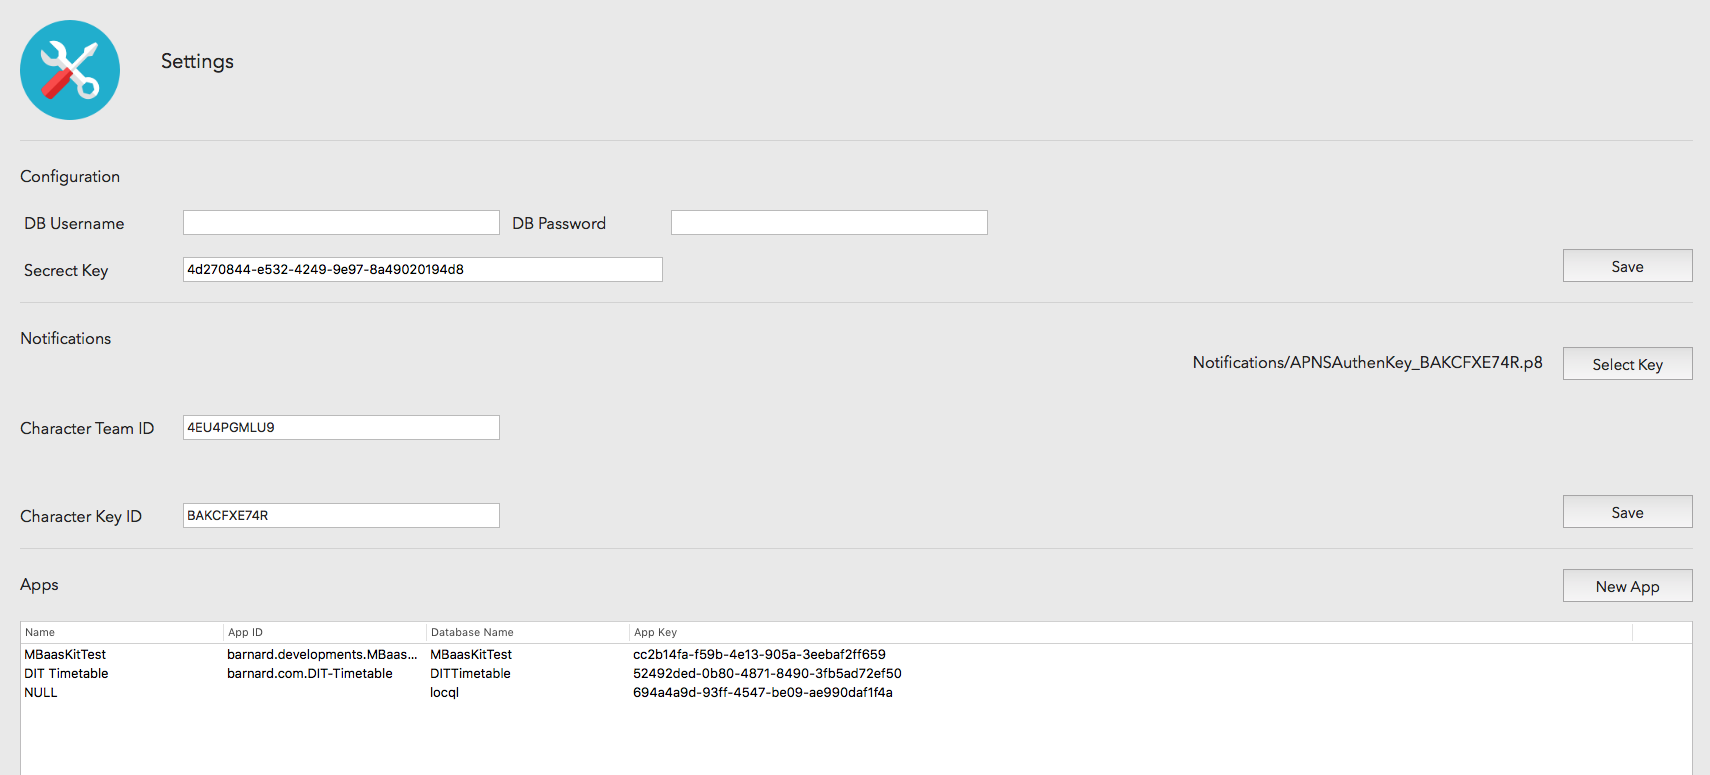
\includegraphics[width=150mm]{images/dashboard/settings}
    \label{fig:settings-view}
\end{figure} 


\begin{figure}[!h]
    \caption{Apps Class Diagram}
    \centering
    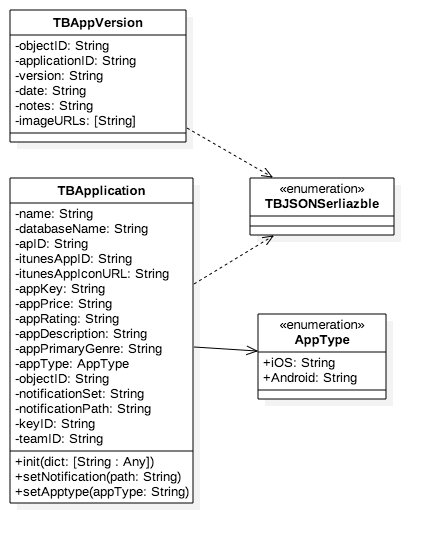
\includegraphics[width=75mm]{images/classdiagrams/Settings}
    \label{fig:settings-cd}
\end{figure} 

Figure \ref{fig:settings-view} illustrates the settings view, where the configuration for the web-server and the mobile applications occurs. The view is split up into three sections; the first section has some configurations values for accessing the web-server and database. The secret key allows the mobile applications to access the web-server so that the key will be put in the header. The database username and password can be set and allows for some extra security.

The notification section is for configuring the Apple Push Notifications (APNs), this has changed in the past year as was mentioned in the design chapter. The process now has sped up to set up the APNs on both the Apple developer console and the server. Now one key file with extension .p8 is all that is required to send APNs, this and three other values. Two of them are the team id, which is the developer's id found in the developer console, and the key id which is provided when requesting a new .p8 key file. The Select Key buttons bring up file window, to get the file from the developer's computer, and uploads the file via HTTP to the server. Once the Save button has been selected, the two values and the key file are sent to the database. The other app id value will be set when an application is being made discussed next.

\begin{figure}[!h]
    \begin{subfigure}{0.5\textwidth}
        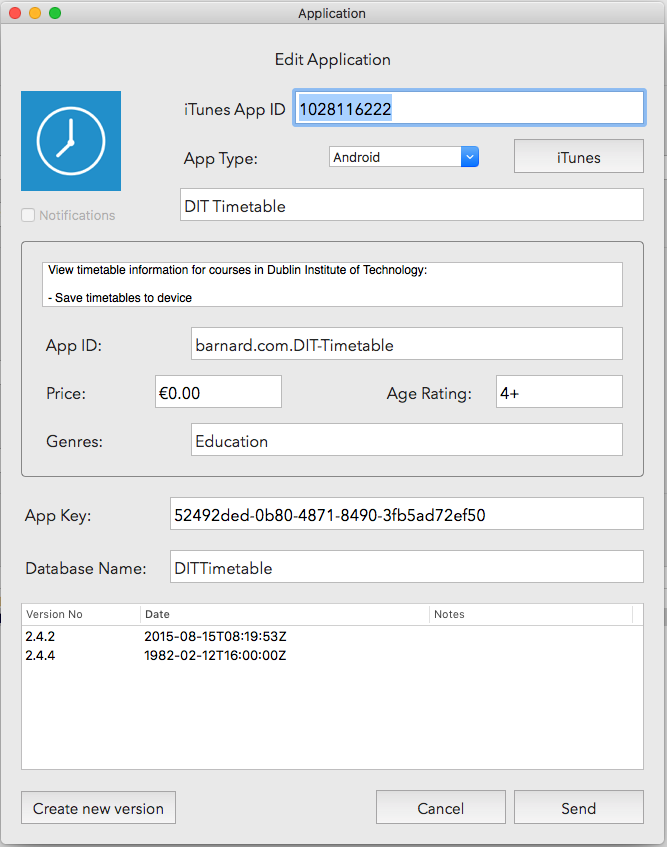
\includegraphics[width=0.9\linewidth, height=10cm]{images/dashboard/newapp}
        \caption{App View}
        \label{fig:subim1}
    \end{subfigure}
    \begin{subfigure}{0.5\textwidth}
        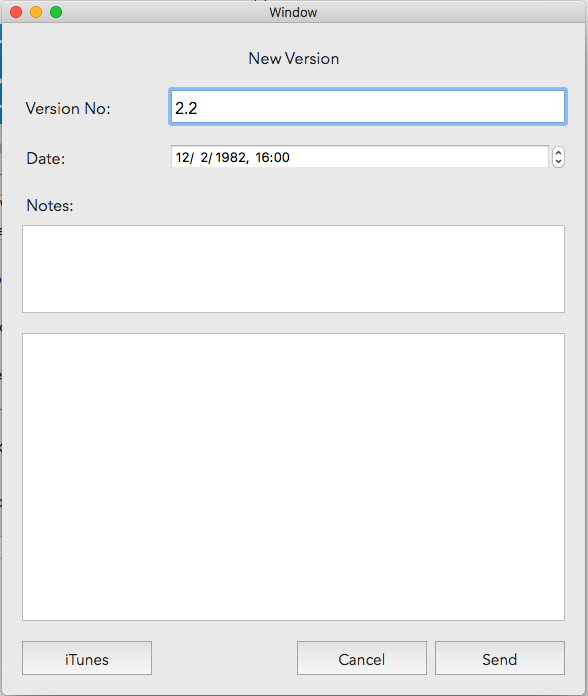
\includegraphics[width=0.9\linewidth, height=10cm]{images/dashboard/newversion}
        \caption{App Version}
        \label{fig:subim2}
    \end{subfigure}
\caption{Configuring Apps}
\label{fig:app-version}
\end{figure}

\begin{figure}[!h]
    \caption{iTunes API}
    \centering
    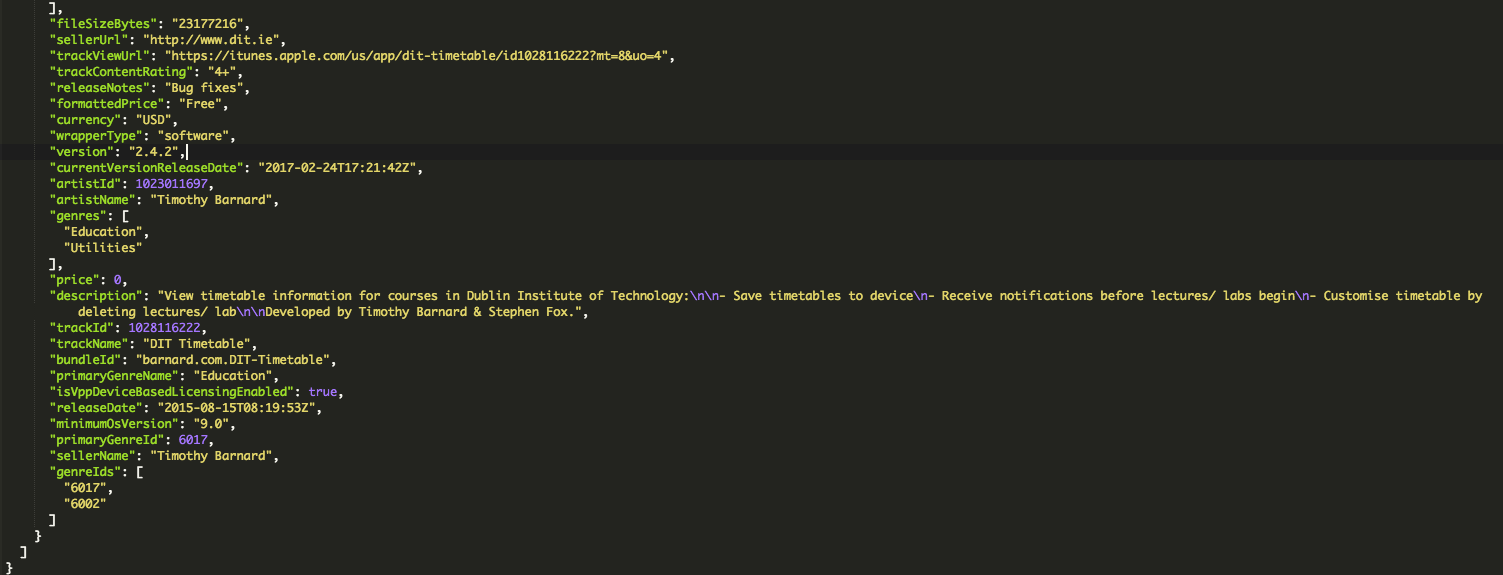
\includegraphics[width=150mm]{images/itunes-api}
    \label{fig:itunes-API}
\end{figure} 

Figure \ref{fig:settings-cd} illustrates the classes for the application and version and Figure \ref{fig:app-version} shows where these values are displayed. Each application contains several properties, and some of these are provided by Apple’s iTunes API. In Figure \ref{fig:subim1}, the button iTunes, once the user has entered the iTunes App ID field, retrieves some values which are displayed inside the box along with the app icon. The URL for making the request is \textit{https://itunes.apple.com/lookup?id=}, and the app id is passed into the GET request, and JSON objects are returned to be parsed into objects as seen in Figure \ref{fig:itunes-API}. After being parsed into iTunes object, these are then set into the TBApplication class to be saved in the database.

This can only be done once the application has been published, but the other fields can be entered until then. The two relevant fields from this view are app key and database name, these are a security feature. Each application gets their database, by doing this keeps the data separate from other applications. The second security feature is the app key; this provides access to the database of the mobile app. As mentioned in the settings section, the secret key is sent up each request; this is also the same with the app key. This was discussed in the server section earlier.

In Figure \ref{fig:subim2}, the developer can keep a history of app versions published. The iTunes API already mentioned does not provide history of published version, so by having the feature gives the developer a history of what changes has been made in each version. This view also displays any notes and app stores images that have been added in that version. The iTunes button at the bottom left does the same as in Figure \ref{fig:subim1}, but this view retrieves different fields to be saved. The reason for this button is that when a new version is published, the app id will return the new app versions data only.

\subsubsection{Staff}

\begin{figure}[!h]
    \caption{Staff View}
    \centering
    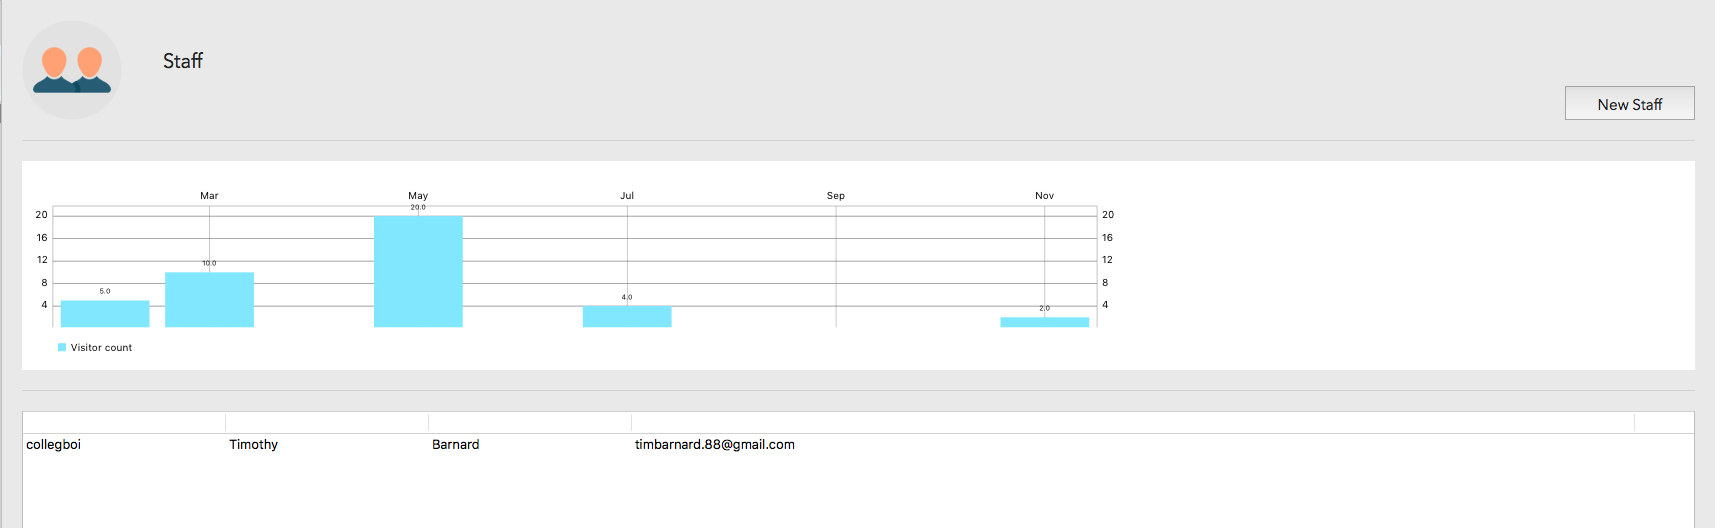
\includegraphics[width=120mm]{images/dashboard/staff}
    \label{fig:staff}
\end{figure} 

\begin{figure}[!h]
    \caption{Edit Staff View}
    \centering
    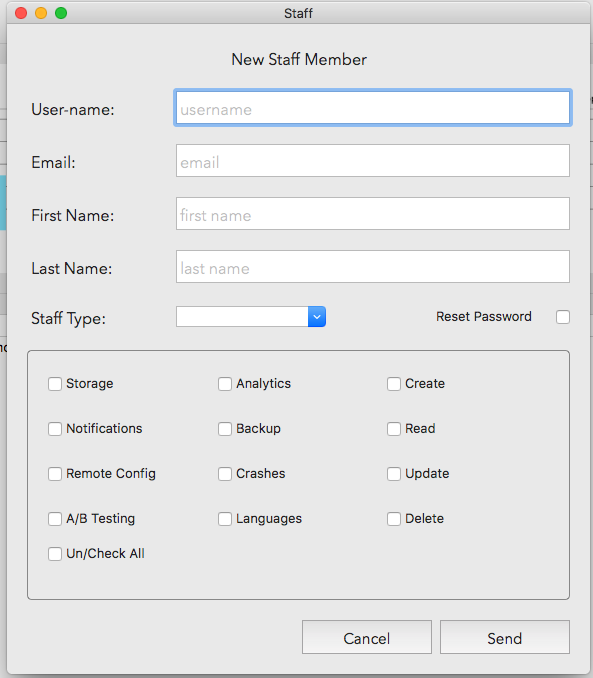
\includegraphics[width=80mm]{images/dashboard/edit_staff}
    \label{fig:edit_staff}
\end{figure} 

The staff view displays all current staff that have been registered as can be seen in Figure \ref{fig:staff}. The bar chart at the top shows the analytics of staff members logging in at a month to month basis. This view allows staff members to be added the \textit{New Staff} button, or edit the current user by clicking the record in the table. Once click, the \textit{Staff Member} window as illustrated in Figure \ref{fig:edit_staff} is displayed where some configurations are to be entered. If the current staff member is of type admin, then the entire window is enabled. The typical details such as username and email address are asked to be entered, but the check boxes inside the box allow the different user rights. The first two columns can be unchecked to limit the user of what is displayed in the side menu. The reset password if the admin is checked for a staff member if they forgot their password.

\subsubsection{Storage}

\begin{figure}[!h]
    \caption{Storage View}
    \centering
    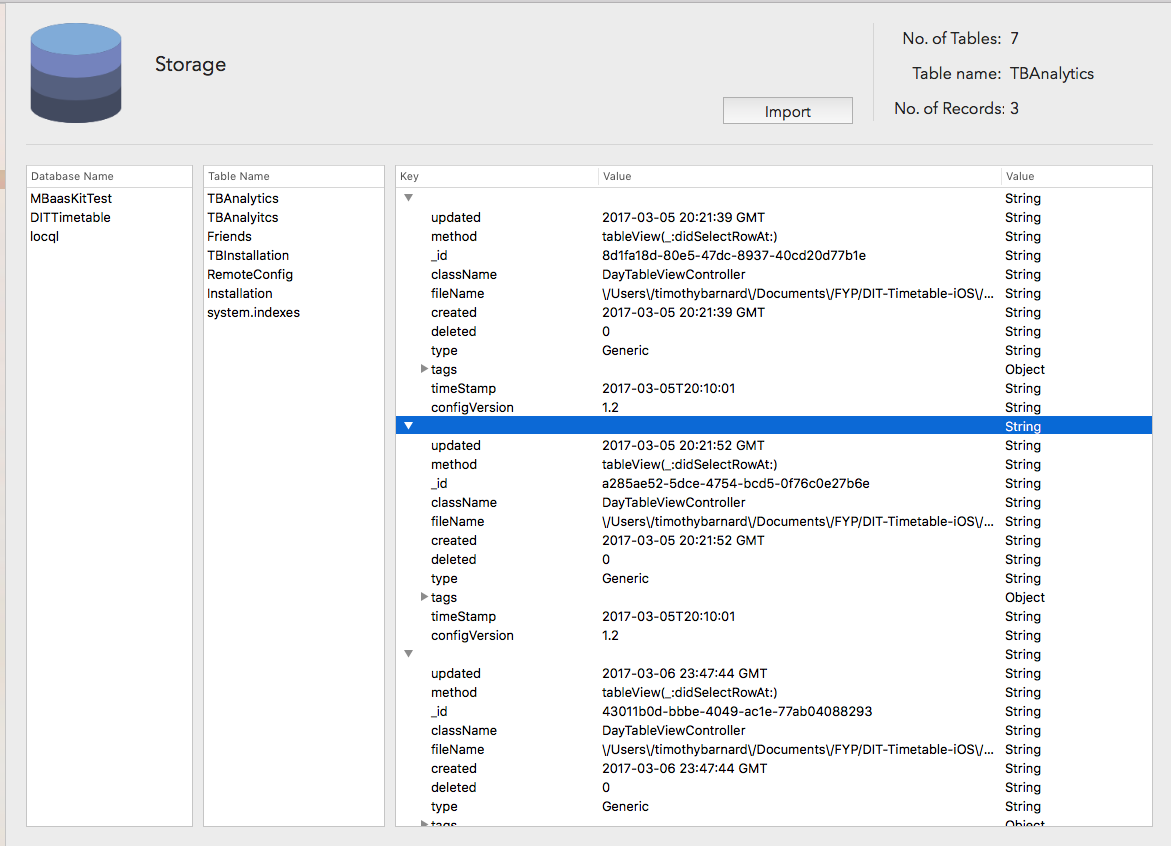
\includegraphics[width=120mm]{images/dashboard/storage}
    \label{fig:storage}
\end{figure}

\begin{figure}[!h]
    \caption{Storage class diagram}
    \centering
    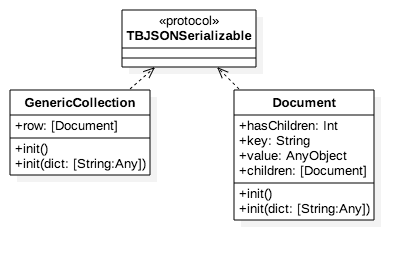
\includegraphics[width=80mm]{images/classdiagrams/storage_class}
    \label{fig:storage_class}
\end{figure} 

The tables illustrated in Figure \ref{fig:storage} display the database contents. The first table contains the list of databases; these are the names that are set out when setting up an application in the settings view. Next once the database name of been chosen, the list of contained collections. The table on the right outputs the contents of the collection, in a parent-child format. So when a cell is clicked, if that parent has children, then it can be expanded to show the values.

The class diagram for the storage view can be seen in Figure \ref{fig:storage_class}, where both classes again conform to the TBJSONSerializable protocol. This class structure is designed to accommodate for any collection of documents retrieved. The \textit{GenericCollection} is the first top class of the collection of records which are contained in the row variable. The row variable is of type Document array, where each Document properties are as follows: \textit{hasChildren} for checking if that parent has children to be able to expand the row, key and value hold the values in each collection document and last the children which contain the list of children as illustrated in Figure \ref{fig:storage}. The \textit{TBAnalytics} collection contains three documents; in one there is key called \textit{tags} which also holds children for example \textit{timeStamp}.

\subsubsection{Analytics}

\begin{figure}[!h]
    \caption{Analytics View}
    \centering
    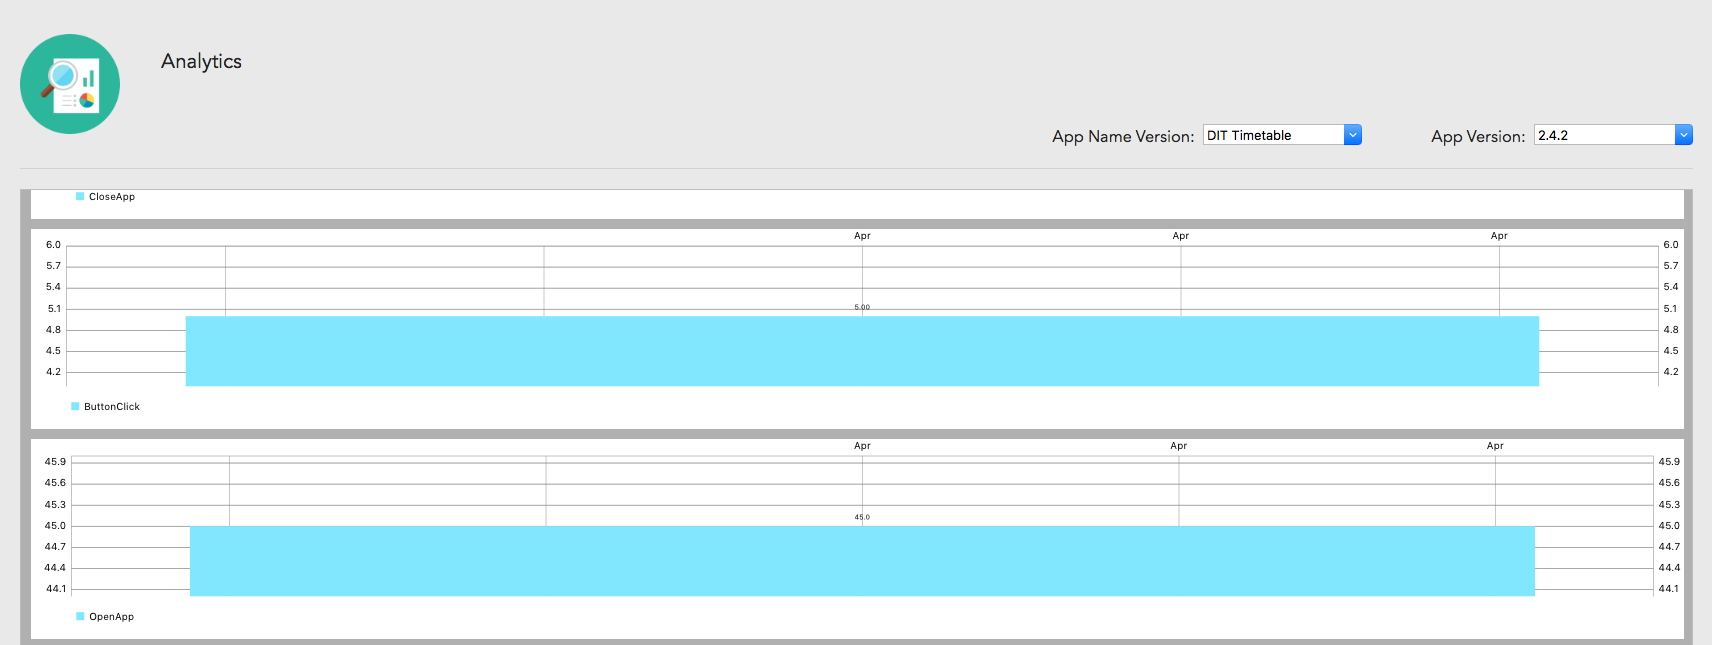
\includegraphics[width=120mm]{images/dashboard/analytics}
    \label{fig:analytics}
\end{figure}

Illustrated in Figure \ref{fig:analytics}, it displays the analytics gathered from the different applications and versions. The drop down lists allows the developer to change where analytics was gathered from. The scroll view below contains a collection of views which display the analytics in a bar chart form. Each bar graph view is for the different types of analytic gathering, as the analytic class diagram can be seen in figure \ref{fig:analytics_class}.

\begin{figure}[!h]
    \caption{Analytics class diagram}
    \centering
    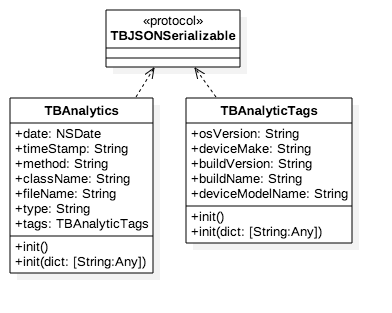
\includegraphics[width=80mm]{images/classdiagrams/analytics_class}
    \label{fig:analytics_class}
\end{figure}

\subsubsection{Languages}

\begin{figure}[!h]
    \caption{Languages View}
    \centering
    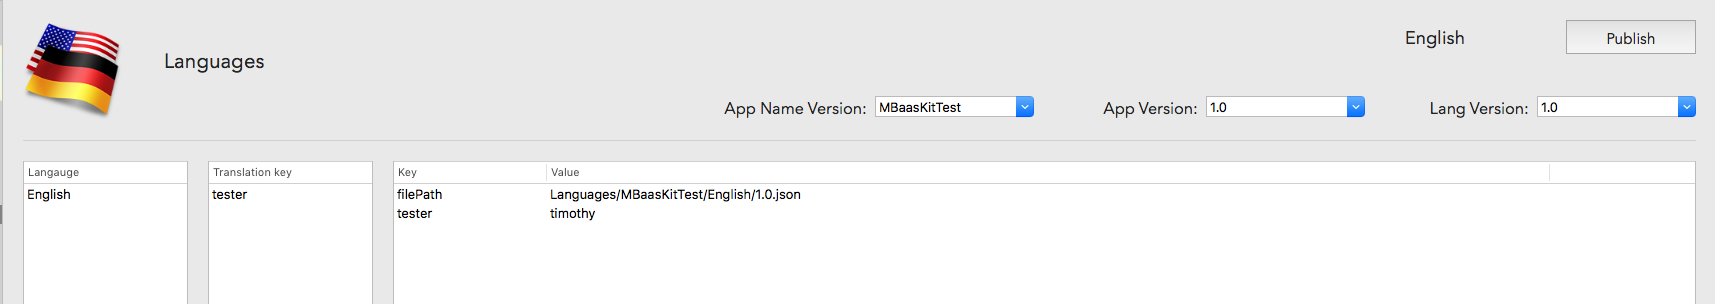
\includegraphics[width=120mm]{images/dashboard/languages}
    \label{fig:languages}
\end{figure} 

The languages view in Figure \ref{fig:languages} illustrates the layout, where the language can be selected, along with creating/updating a translation. After the mobile app and version have been chosen, the languages and translations will be displayed in the tables below. The first table shows the current languages which can be changed to active/inactive as required, which can limit if a language is an option. The next table is a collection of keys (translation keys) that is available, by separating this enables the developer to see what other translations have. This will remove any discrepancy’s between the translations files, e.g., between English and French.

\begin{figure}[!h]
    \caption{Language class diagram}
    \centering
    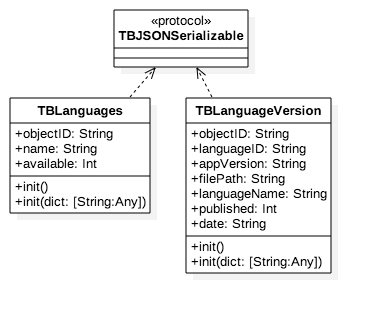
\includegraphics[width=80mm]{images/classdiagrams/lang_class}
    \label{fig:lang_class}
\end{figure}

Figure \ref{fig:lang_class} shows the class diagram which is used in the Language View. The languages class holds properties including the name, for example, English, and if that language is available in the currently selected version of the app. The language version class is where the meta-data regarding each version of translation are kept. These include the app version, the file path to the location where the language file is being stored, and if this version is published.

\subsubsection{Notifications}

\begin{figure}[!h]
    \caption{Storage View}
    \centering
    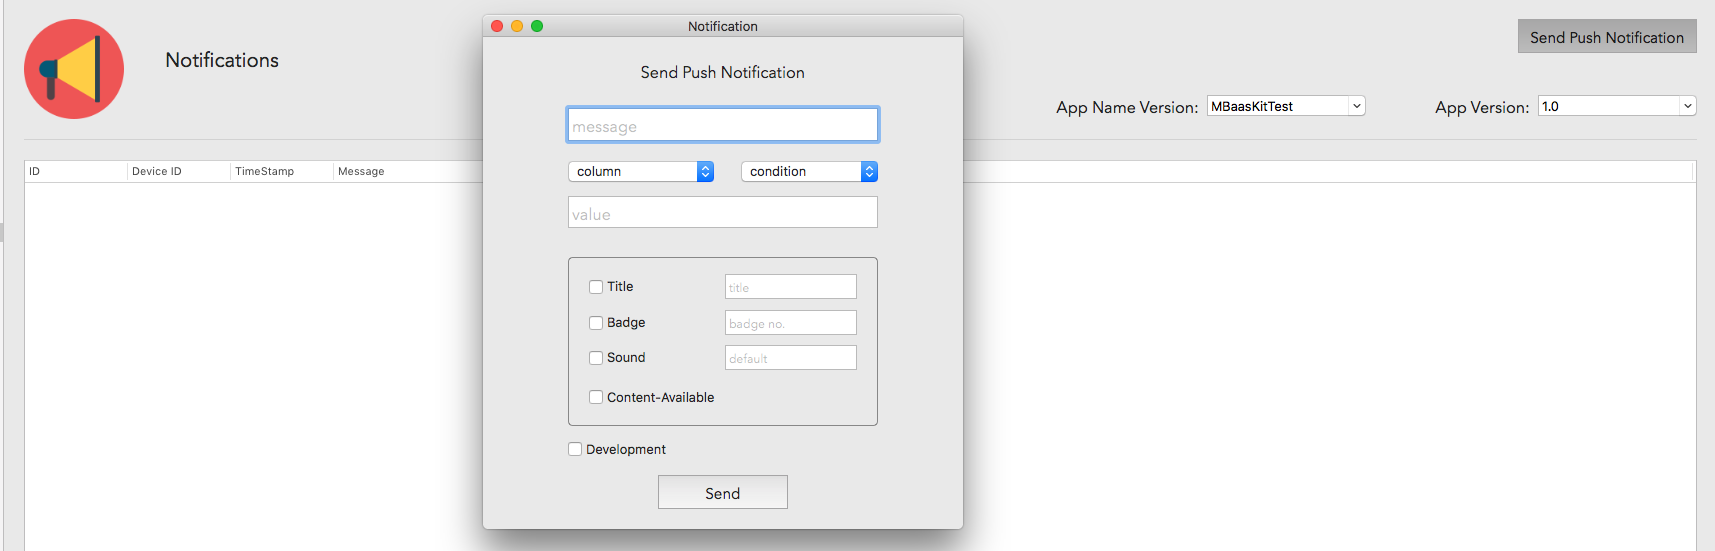
\includegraphics[width=120mm]{images/dashboard/notifications}
    \label{fig:notification}
\end{figure}

The notification view in Figure \ref{fig:notification} has two functionalities, one for view all sent notifications, and the other two send one manually. This can be done by selecting Send Push Notification button at the top right, which will bring up a new window. The fields that can be entered are what are used when sending notifications, and the two main ones are the message itself and the unique device id. The window also supports the capability of sending multiple notifications to all devices or grouped by device type, etc. The fields inside the box are optional, the title of the notification and if not set is the application name. Once the send button is pressed, a request is made to the web server to send the notifications now.

\subsubsection{Remote Configuration}

\begin{figure}[!h]
    \caption{Remote Configuration View}
    \centering
    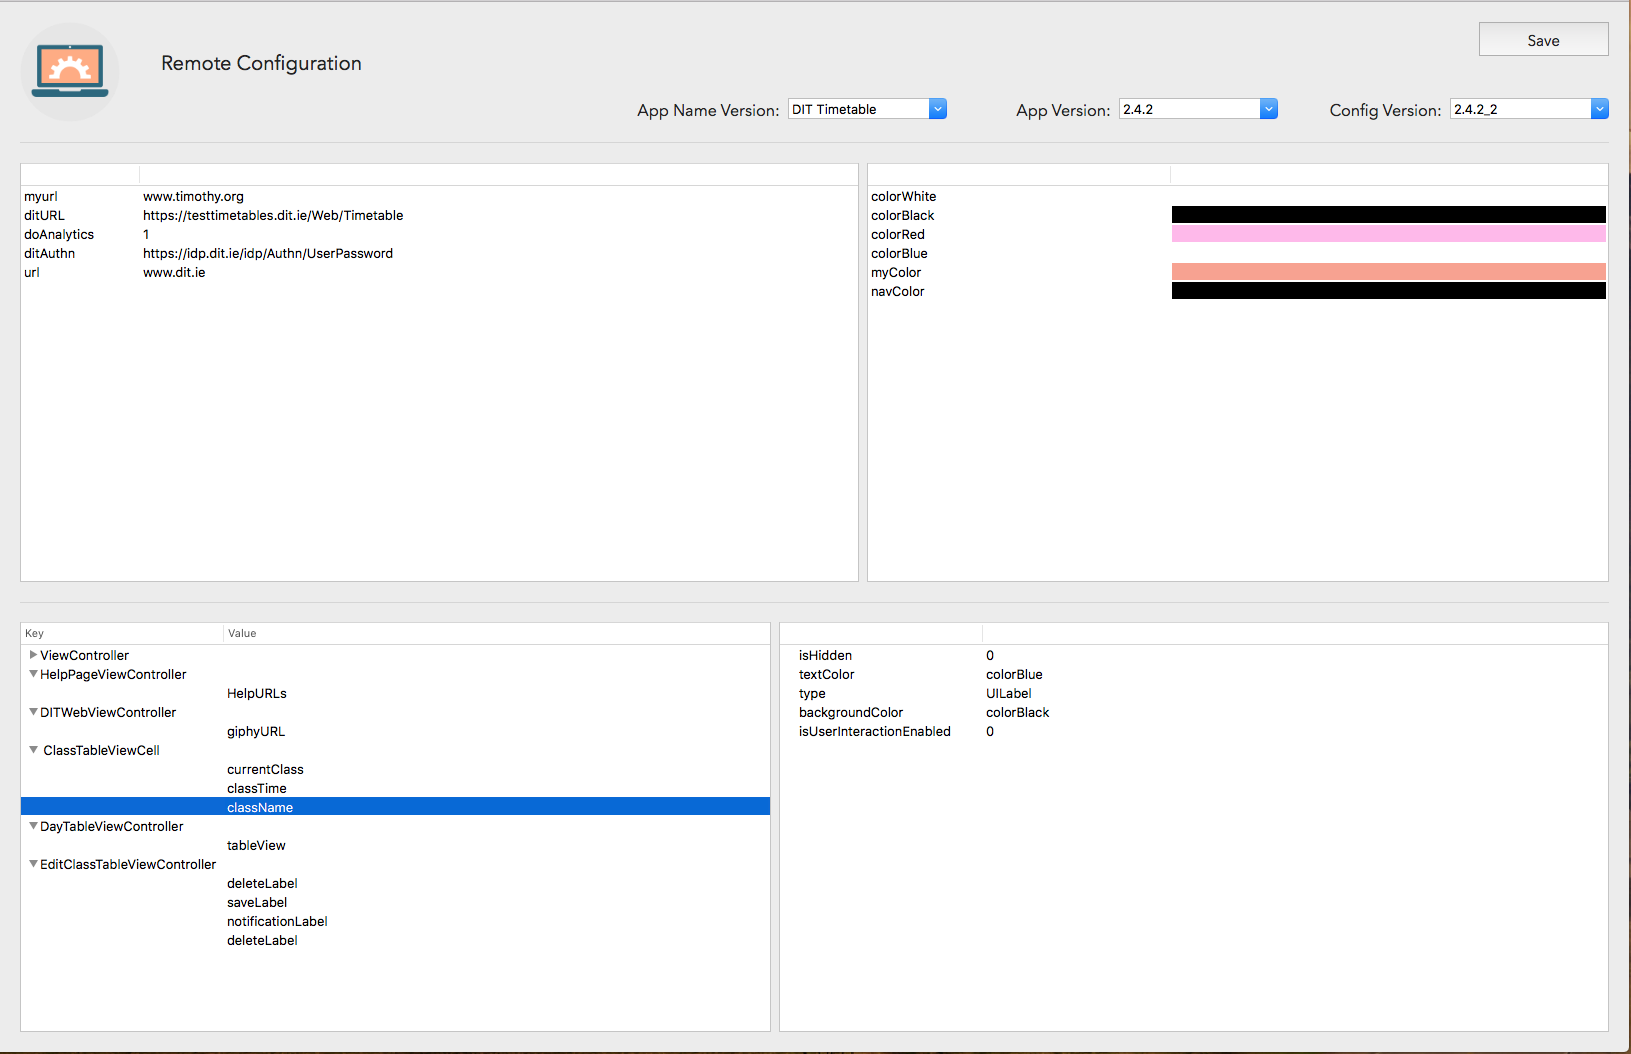
\includegraphics[width=150mm]{images/dashboard/remote-config}
    \label{fig:remote-config-view}
\end{figure}

\begin{figure}[!h]
    \caption{Remote Configuration View}
    \centering
    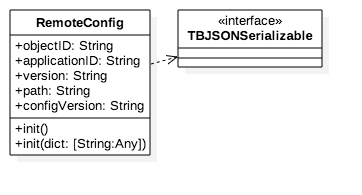
\includegraphics[width=80mm]{images/classdiagrams/RemoteConfig}
    \label{fig:remote-config-cd}
\end{figure} 

The remote configuration view as illustrated in Figure \ref{fig:remote-config-view} contains four tables which in turn represents the four classes already discussed in the services section in Figure \ref{fig:rc-cd}. The figure displays the current configuration for the DIT-Timetable app with version 2.4.2. When the page initially loads, the first of each drop down list is chosen to show that current configuration. The first of the drop down menus display the list of applications, which are taken from TBApplication collection. This collection is set from the settings to view already discussed, along with the application versions, which is the contents of the next drop down. The last list contains the current configuration versions as seen in Figure \ref{fig:remote-config-cd}. Each remote configuration object has an application and version, its relates to. The configVersion property allows for A/B Testing service which is discussed next.

Starting from the top left table which contains the main settings values, next on the right at the colours used in that particular version of the app. The bottom left table contains the view controller or classes, and if a class contains objects, the cell can be expanded to display all the objects. Once an object has been selected, the table on the right provides all possible properties that can be used. This part of the dashboard also contains a JSON file, that contains all UI objects that can select with their properties as illustrated in Listing \ref{lst:label_json}. If a property options are a list type, then the raw string values are shown, for example, textAlignment. In Swift, the UI object property options are the type of enumeration, so when the user chooses an option, the integer value is stored. When a property has been selected, either two of views will show as illustrated in Figure \ref{fig:property1}. The value can then selected and set.

\lstinputlisting[label={lst:label_json}, caption=UI Object JSON]{development/code/Label_json.m}

\begin{figure}[!h]
    \caption{Edit Property View}
    \centering
    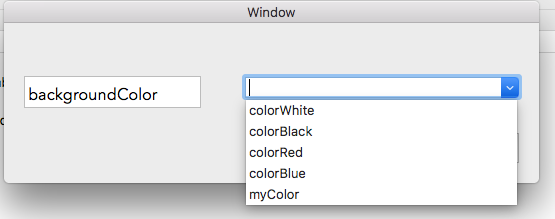
\includegraphics[width=80mm]{images/dashboard/property-1}
    \label{fig:property1}
\end{figure} 

\begin{figure}[!h]
    \caption{Save Configuration View}
    \centering
    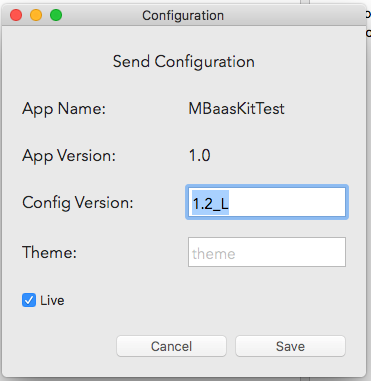
\includegraphics[width=80mm]{images/dashboard/configuration}
    \label{fig:configuration}
\end{figure} 

Once the configuration has been set, the user has the option to save and publish that version. This can be done by pressing the Save button at the top right which displays a new window as illustrated in Figure \ref{fig:configuration}. This view allows the user to set the version name and theme. The testing chapter will demonstrate the configuration of the theme in use. The live check box if unchecked can restrict this version for the mobile application to use.

\subsubsection{AB Testing}

\begin{figure}[!h]
    \caption{AB Testing View}
    \centering
    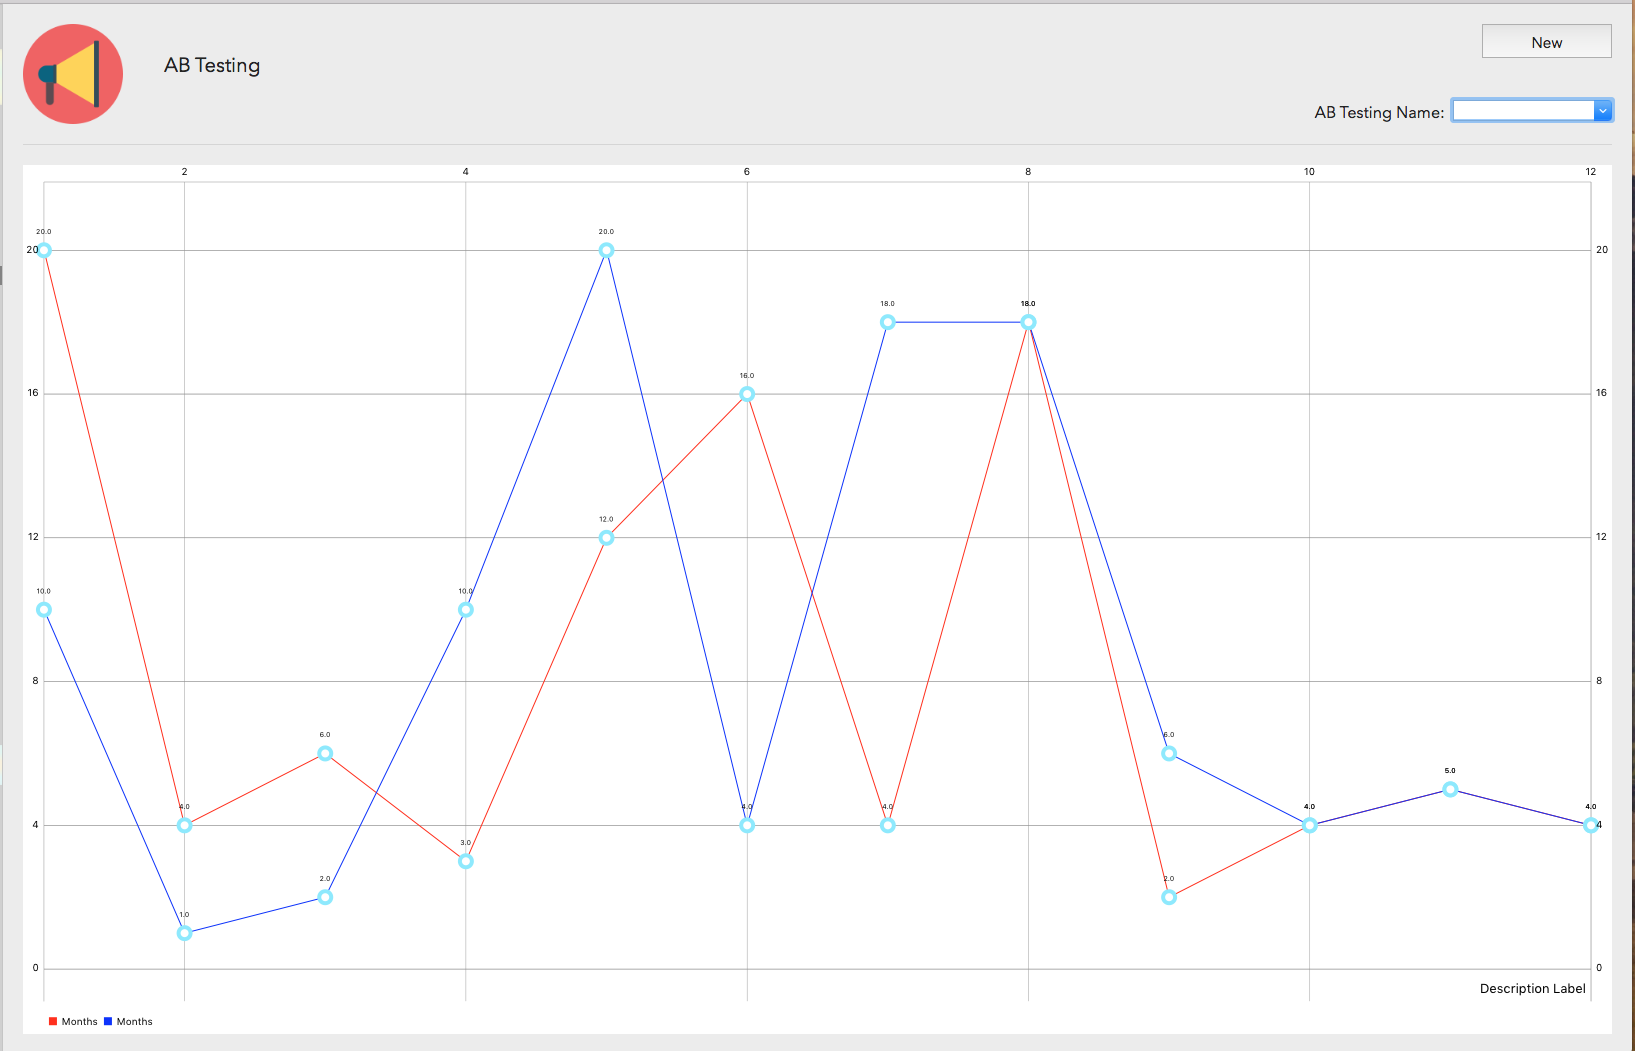
\includegraphics[width=120mm]{images/dashboard/abtesting}
    \label{fig:abtesting-view}
\end{figure} 

\begin{figure}[!h]
    \caption{AB Testing Config View}
    \centering
    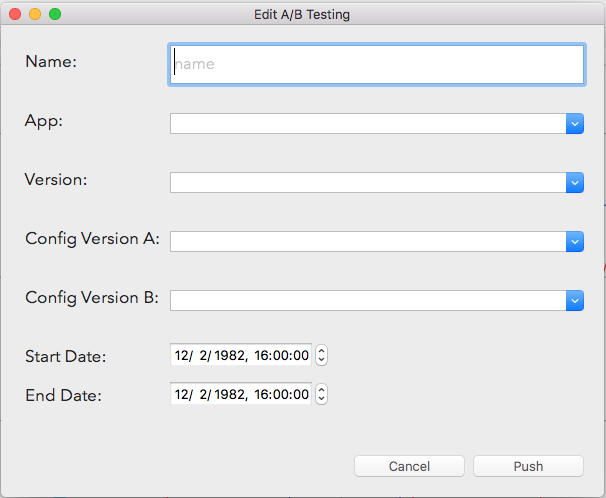
\includegraphics[width=100mm]{images/dashboard/abtesting-config}
    \label{fig:abtesting-config-view}
\end{figure} 

Figure \ref{fig:abtesting-view} illustrates the AB Testing view, and figure \ref{fig:abtesting-config-view} shows how to configure the A/B testing object. The main AB testing view displays a line chart with two line. Each line corresponds to a version that has been included in a particular testing set up, as was already discussed with Figure \ref{fig:abtesting-cd}. The analytical data gathered is from the \textit{TBAnalytics} class that was examined in section analytics.

The drop-down list can be used to select a particular testing, and view the results to see what configuration version had the highest usage. To configure a new A/B testing, the new button is pressed to display the new in Figure \ref{fig:abtesting-config-view}. The following values are required to be set, the name, the application name, the particular version of the app and the next two drop down list are the different versions that were already configured in Remote Configuration view. The start and end time are set to allow a period for which these tests are run. Once all the values have been entered, the push button will send the new object to the database, and when a request is made to the server for a configuration file, the A/B testing object will be retrieved, and one of the versions will be shown.

\subsubsection{Backup}

\begin{figure}[!h]
    \caption{Backup View}
    \centering
    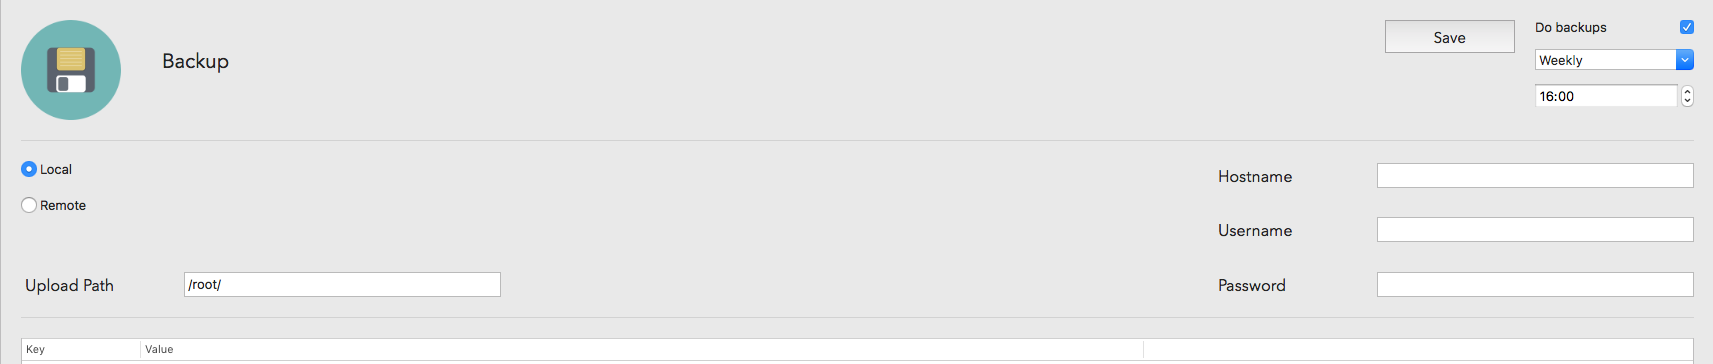
\includegraphics[width=150mm]{images/dashboard/backup}
    \label{fig:backup-view}
\end{figure} 

Figure \ref{fig:backup-view} illustrates the backup view, where completed backup of the database and files can be configured. This view offers a list of configurable values, including if backups are to be done in the first place. Once checked, the drop down list can be set to daily, weekly or a particular day of the week. Next, the time of the backup can be configured; then the developer has two options to save the backups locally or remotely. If locally the folder path only needs to be entered.

Each backup folder name will contain the timetamp of when the backup occurred. After the configuration has to be done, the save button will send the values to the server and start the process. In the web-server section later, the backup web app will be discussed in detail of what happens. The table to the bottom will contain a list of backups that have been done, and by right clicking a record and clicking Delete, both the record and the backup directory will be deleted.

\subsubsection{Issues}

\begin{figure}[!h]
    \caption{Issues View}
    \centering
    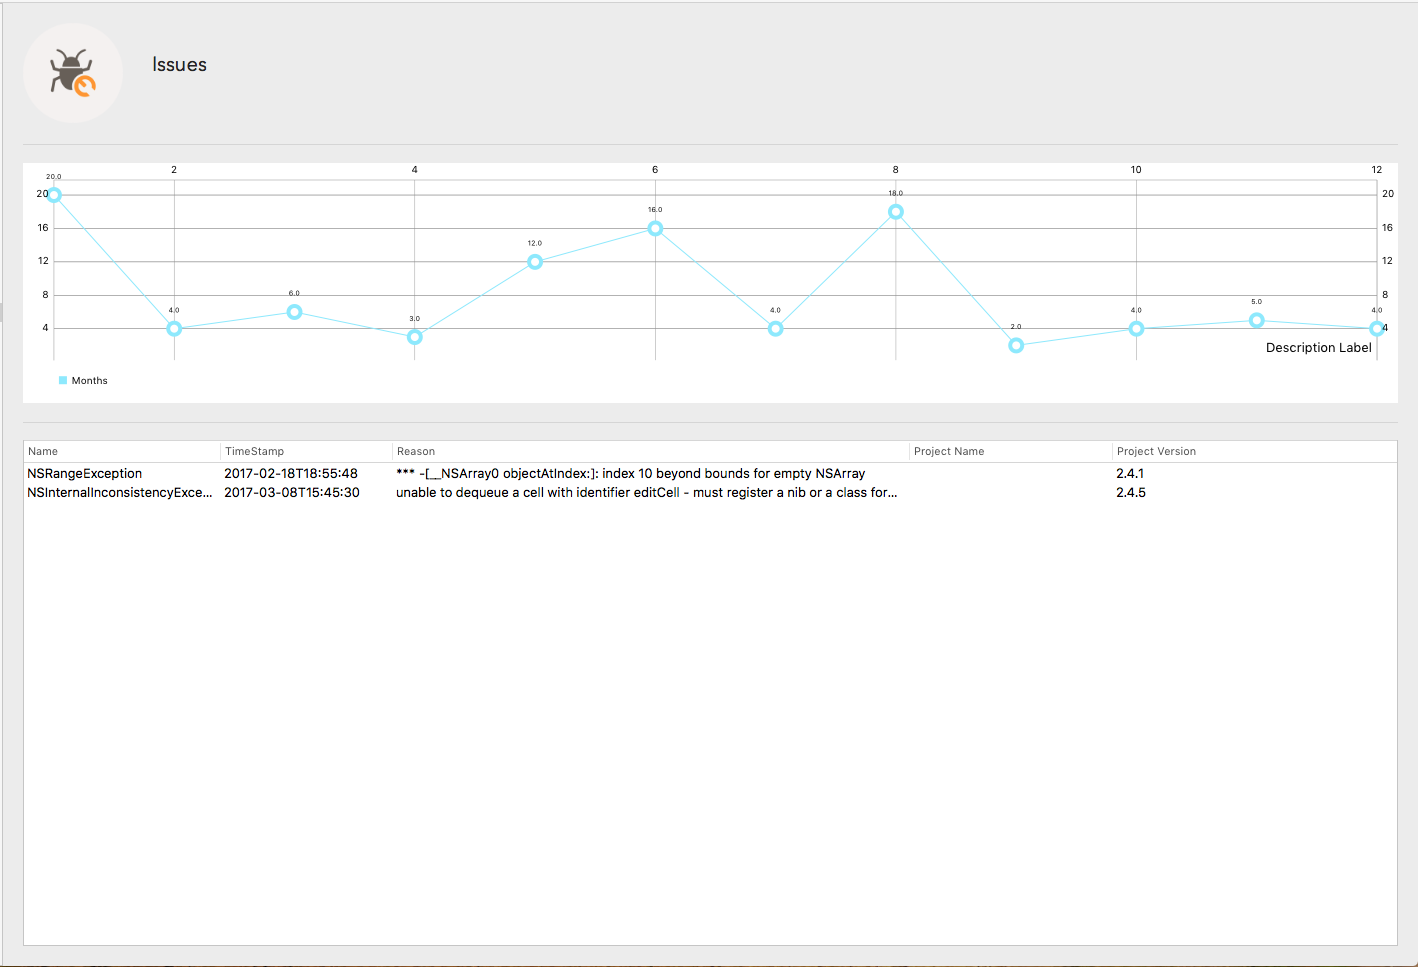
\includegraphics[width=150mm]{images/dashboard/crashes}
    \label{fig:crashes-view}
\end{figure} 

\begin{figure}[!h]
    \caption{View Detailed Issue}
    \centering
    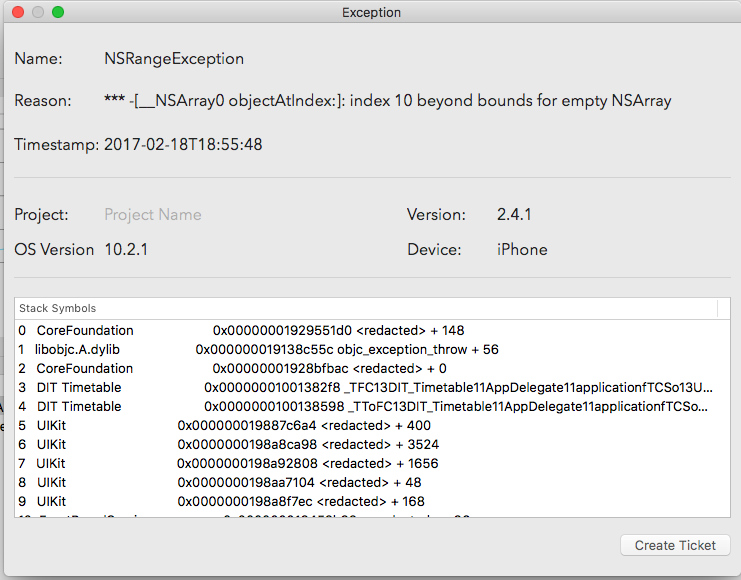
\includegraphics[width=150mm]{images/dashboard/view_crash}
    \label{fig:view-crash}
\end{figure} 

The issue view as illustrated in Figure \ref{fig:crashes-view} is where all exceptions from the mobile applications are displayed. The line chart shows the number of exceptions on a 12-month basis. This can give the developer a quick overview of how the application is doing. The exception class structure was already discussed in the services section. If the table below displays any exceptions, the record can be clicked to show the exception in more detail as can be seen in Figure  \ref{fig:view-crash}. In this window, the issue can be attached to a new ticket which is discussed next.

\subsubsection{Tickets}

\begin{figure}[!h]
    \caption{Tickets View}
    \centering
    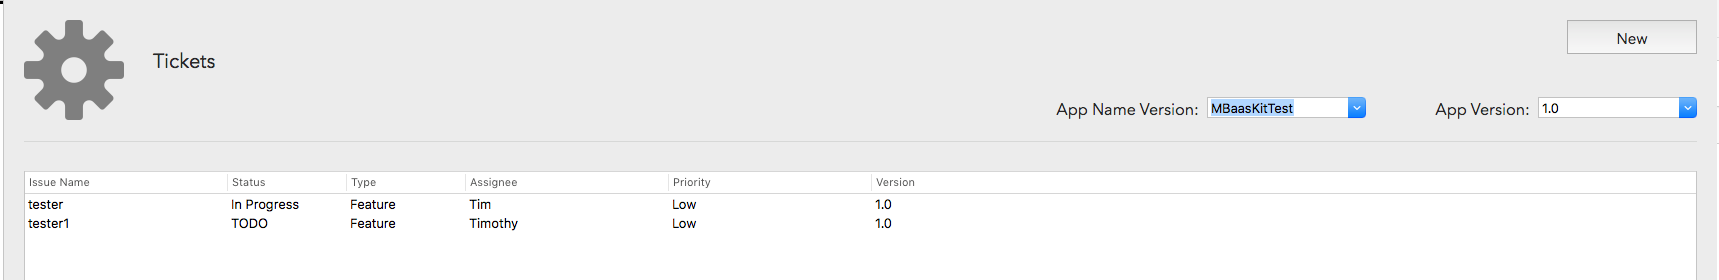
\includegraphics[width=150mm]{images/dashboard/tickets}
    \label{fig:issues-view}
\end{figure} 


\begin{figure}[!h]
    \caption{Issues Class Diagram}
    \centering
    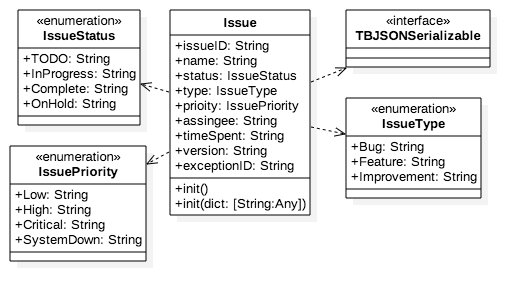
\includegraphics[width=100mm]{images/classdiagrams/Issues}
    \label{fig:issues-cd}
\end{figure} 

Figure \ref{fig:issues-view} illustrates the tickets view containing all the different type of tickets being, bugs, features, etc. are displayed. After selecting the application name and version from the drop-down list, the table below will get populated with the current issues relating to that application. The class diagram for each issue is illustrated in Figure \ref{fig:issues-cd}, where the Issue class has the same protocol again. This gives the class functionality to save and retrieve all the issues. The issue class consists of few enumeration type variables, where an issue can be a bug, the issue has a status and priority. An enumeration was used to make sure of the value being parsed into the database, being only one of the values.

\begin{figure}[!h]
    \caption{Tickets View}
    \centering
    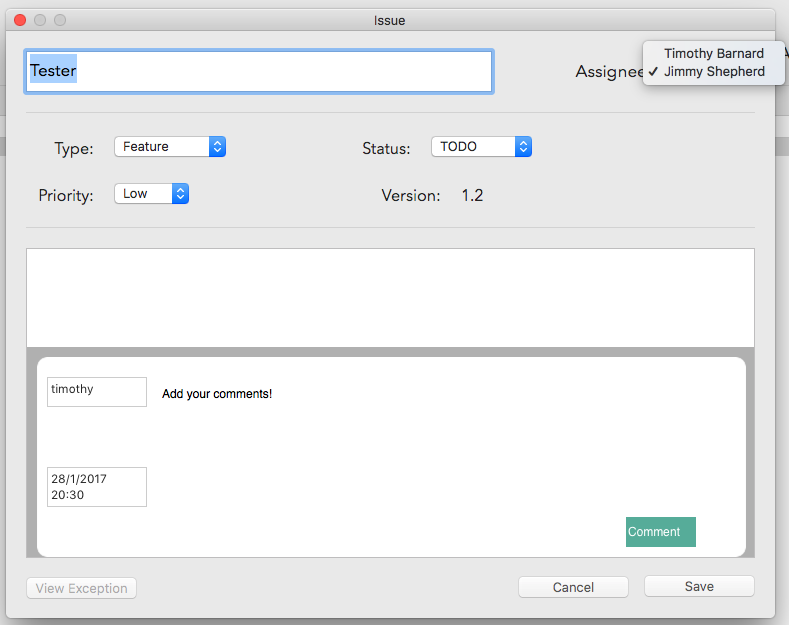
\includegraphics[width=100mm]{images/dashboard/edit_issue}
    \label{fig:edit_issue-view}
\end{figure} 


To be able to create a new and edit an issue, a new window was developed. This view as seen in Figure \ref{fig:edit_issue-view} contains several values, starting off with the name of the ticket, and the assignee. The issue displayed has a type of feature, the status of \textit{TODO} and low priority and the app version. The \textit{"Add your comments"} section contain the logged comments regarding this ticket, which can be done several times. Each recorded comment will include the assignee and the timestamp.

\subsubsection{Sprint Board}

\begin{figure}[!h]
    \caption{Sprint Board View}
    \centering
    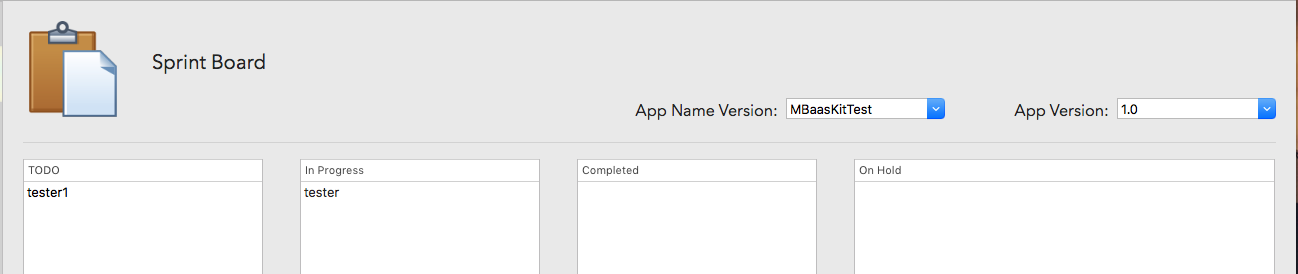
\includegraphics[width=150mm]{images/dashboard/sprint-board}
    \label{fig:sprint-board-view}
\end{figure} 

Figure \ref{fig:sprint-board-view} illustrates the sprint board view, where the tickets/issues from the previous section will show. This view gives the developer an easier layout to monitor when working through assigned tickets. The issues can also be dragged and moved into a different table, so moving an issue from in progress section to completed. The main function for this can be seen in Listing \ref{lst:sprint}, which looks after moving the value into the correct table.

\lstinputlisting[label={lst:sprint},language=Swift, caption=Sprint]{development/code/sprint.m}

\section{CocoaPod Framework}

First, the CocoaPod was initialised, and this was done all on the command line as see in Listing \ref{lst:pod_init}. The first command installs CocoaPods, then once installed, the pod is created. The \textit{pod lib lint} builds the skeleton structure and associated files, next to create the project; \textit{pod lib creates MBaaSKit} was run which was followed by the terminal asking for some inputs.

\lstinputlisting[label={lst:pod_init}, language=Bash, caption=Pod Init]{development/code/pod_init.m}

\begin{itemize}
  \item What language do you want to use?
  - Swift
  \item Do you want to include demo application?
  - Yes
  \item What testing framework do you use?
  - None (this will be done later)
  \item Do you want to view based testing?
  - No
\end{itemize}

After the pod is initialised, the .podspec file required to be updated, so running \textit{nano MBaaSKit.podspec} to edit the file. The following values are needed to be updated: 

\begin{itemize}
  \item s.summary
  - a brief summary of the pod
  \item s.description
  - a brief description of the pod
  \item s.homepage
  - Github link to the location of the pod
\end{itemize}

After the pod has been setup, the next listing \ref{lst:pod_git} adds all the files and commits to local origin repository and pushes to master.

\lstinputlisting[label={lst:pod_git}, language=Bash, caption=Pod Github]{development/code/pod_git.m}

At this stage, the pod has been set up, and the initial Github commit has been pushed. 

Once the project files and code has added, the next stage was to make the pod available known as pod tagging. This was done by running the following commands in Listing \ref{lst:pod_tagging}. The first command git tag "0.0.1" was run, which gives a version, then git push origin "0.0.1". After which pod spec lint MBaaSKit.podspec verifies that everything is configured correctly between where the source code is stored and the .podspec file. The output states "MBaaSKit.podspec passed validation", so the last command to push the pod can be done. 

\lstinputlisting[label={lst:pod_tagging}, language=Bash, caption=Pod Tagging]{development/code/pod_tagging.m}

The classes to be used in the library has already been implemented in the services section. The services have gone through design and testing, and now can be added to the Cocoapods framework. The classes and class functions had to be updated with the public keyword. This public keyword gives the mobile app access to these files, and this library is technically outside the project. This SDK is tested using another mobile app; this will be discussed in the testing chapter.

\section{Conclusion}

The project development was a challenging part, with not knowing the suggestive improvements would work.

\subsection{Code Stats}

\begin{table}[!h]
\centering
\caption{Project Code Stats}
\label{my-label}
\begin{tabular}{|l|l|l|}
\hline
\rowcolor{green!20}
Deliverable & Files & Code   \\ \hline
Server      & 33    & 2,663  \\ \hline
Dashboard   & 264   & 27,507 \\ \hline
SDK         & 36    & 2,271  \\ \hline
Total       & 333   & 29,778 \\ \hline
\end{tabular}
\end{table}